\documentclass[doublespace,Afour,sageh,times]{sagej}
\usepackage{amsmath,amssymb,amsthm,mathtools,graphicx,booktabs,array,url,tabularx,multirow}
\usepackage{microtype,etoolbox}
\usepackage{xr-hyper}
\usepackage[colorlinks,bookmarksopen,bookmarksnumbered,citecolor=blue,urlcolor=blue,linkcolor=blue]{hyperref}
\setcounter{secnumdepth}{3}
\setcounter{dbltopnumber}{2}
\renewcommand{\dbltopfraction}{0.90}
\renewcommand{\textfraction}{0.08}
\renewcommand{\floatpagefraction}{0.8}
\emergencystretch=2em
\renewcommand{\bibfont}{\fontsize{9}{11pt}\selectfont}
\setlength{\tabcolsep}{4pt}
\newcolumntype{Y}{>{\raggedright\arraybackslash}X}
\def\journalname{V10 integrated revision}
\def\volumenumber{1}
\def\issuenumber{EN}
\newcommand{\versionlanguage}{English master}
\runninghead{Birkhoff discretization and residual control}
\newtheorem{theorem}{Theorem}
\newtheorem{proposition}[theorem]{Proposition}
\newtheorem{lemma}[theorem]{Lemma}
\newtheorem{corollary}[theorem]{Corollary}
\theoremstyle{definition}
\newtheorem{assumption}{Assumption}
\newtheorem{remark}{Remark}
\newcommand{\R}{\mathbb R}
\newcommand{\C}{\mathbb C}
\newcommand{\T}{\mathbb T}
\newcommand{\dd}{\,\mathrm d}
\newcommand{\norm}[1]{\left\lVert#1\right\rVert}
\newcommand{\abs}[1]{\left|#1\right|}
\newcommand{\diag}{\operatorname{diag}}
\newcommand{\Rea}{\operatorname{Re}}
\newcommand{\Ima}{\operatorname{Im}}
\newcommand{\eps}{\varepsilon}
\providecommand{\doi}[1]{\href{https://doi.org/#1}{doi: #1}.}
\makeatletter
\def\@maketitle{%
\if@Royal
\vspace*{-20pt}
\fi
\if@Crown
\vspace*{-20pt}
\fi
\vspace*{-34pt}%
\null%
\begin{center}
\if@PCfour
\begin{rm}
\else
\begin{sf}
\fi
\begin{minipage}[t]{\textwidth-57.625mm}
  \vskip 12.5pt%
    {\raggedright\titlesize\textbf{\@title} \par}%
    \vskip 1.5em%
    \vskip 12.5mm%
    \end{minipage}\hspace{15mm}\begin{minipage}[t]{42.625mm}
\hbox{}\scriptsize\journalname\\
\hbox{}Direction I framework integration\\
\hbox{}28 October 2026\\
\hbox{}\versionlanguage\\[4pt]
\hbox{}{\fboxsep 2pt\fbox{Research draft}}
\end{minipage}
{\par\large%
\if@Royal
      \vspace*{6mm}
      \fi
      \if@Crown
      \vspace*{6mm}
      \fi%
      \lineskip .5em%
      {\raggedright\textbf{\@author}
      \par}}
     \vskip 40pt%
    {\noindent\usebox\absbox\par}
    {\vspace{20pt}%
      %
      {\noindent\normalsize\@keywords}\par}
      \if@PCfour
      \end{rm}
      \else
      \end{sf}
      \fi
      \end{center}
      \if@Royal
      \vspace*{-4.5mm}
      \fi
      \if@Crown
      \vspace*{-4.5mm}
      \fi
      \vspace{22pt}
        \par%
  }
 
\makeatother


\externaldocument{main_xr}[v10_Integrated_EN.pdf]
\runninghead{Supplementary mechanics, proofs and reproducibility}
\renewcommand{\thesection}{S\arabic{section}}
\renewcommand{\theequation}{S\arabic{equation}}
\renewcommand{\thetheorem}{S\arabic{theorem}}
\renewcommand{\theassumption}{S\arabic{assumption}}
\renewcommand{\theremark}{S\arabic{remark}}
\renewcommand{\thetable}{S\arabic{table}}
\renewcommand{\thefigure}{S\arabic{figure}}
\hypersetup{pdftitle={Supplement: Birkhoff discretization and complex Hamiltonian residual control of a magnetic catheter model},pdfauthor={Anonymous authors}}
\begin{document}
\title{Supplementary material: Birkhoff discretization and complex Hamiltonian residual control of a magnetic catheter model}
\author{Anonymous authors}
\begin{abstract}
This supplement provides the mechanics, endpoint and matrix derivations, controlled-map identities, learning-error bounds and reproduction protocols for the three-subproblem article. The same revised beam and endpoint magnet are used throughout. Detailed formulas distinguish the matrix implementation, residual compensation and finite-time controlled convergence from the additional hypotheses of discrete KAM. A separate final section retains learned-reference tracking as a related extension; it does not replace the compensation objective analyzed in the main article. Source provenance and a framework-to-section map accompany the reproducible project.
\end{abstract}
\keywords{supplementary derivations, parameter provenance, numerical verification, reproducibility}
\maketitle
\raggedbottom
\section{Mechanical derivation and parameter traceability}\label{sec:supp-mechanics}
\subsection{General rod reduction and force accounting}
\label{sm:general}
For a spatial rod, define reference strains and body angular velocity by
\begin{equation}
 \Gamma=D^{\mathsf T}r_s,\qquad
 D_s=D\widehat\kappa,\qquad
 D_t=D\widehat\omega_b.
 \label{sm:rod-kinematics}
\end{equation}
The hat map satisfies $\widehat a b=a\times b$.
The spatial balance laws are
\begin{align}
 \rho A_c r_{tt}&=n_s+f_{\rm mag}+f_{\rm h}+f_{\rm c}+\rho A_c g,\\
 \partial_t(D\mathcal J_b\omega_b)&=m_s+r_s\times n+\tau_{\rm ext}.
 \label{sm:rod-balances}
\end{align}
Here $\mathcal J_b$ is the rotational inertia per unit reference
length. For constant body inertia, the second left-hand side equals
$D(\mathcal J_b\dot\omega_b+\omega_b\times\mathcal J_b\omega_b)$.
A stored-energy density determines the unconstrained force and moment
components through its strain derivatives \citep{simo,antman}.
In an unshearable specialization, the eliminated shear strains have
constraint reactions; setting those strains to zero in an unconstrained
shear law does not set the transverse internal forces to zero.

A body-fixed moment density $m_b(s)$ in a static applied field has
potential
\begin{equation}
 V_{\rm mag}=-\int_0^L (Dm_b)\cdot B_0(r)\dd s.
 \label{sm:distributed-magnetism}
\end{equation}
The point-dipole benchmark replaces this distribution by a distal
localized core. The permanent-dipole formulas are the leading terms of
a localized magnetic stress resultant \citep{abbott}. In a surrounding
vacuum region, the Maxwell stress is
\begin{equation}
 T_M=\mu_0^{-1}\left(BB^{\mathsf T}-\tfrac12|B|^2I\right).
 \label{sm:maxwell-stress}
\end{equation}
Its surface force and moment use the total field. Equivalently, for a
complete localized steady current $j(\xi)$, including bound currents,
and externally generated $B_{\rm ext}$,
\begin{align}
 m_d&=\tfrac12\int \xi\times j(\xi)\dd V,\nonumber\\
 F&=\nabla_r[m_d\cdot B_{\rm ext}(r)]+R_F,\nonumber\\
 \tau&=m_d\times B_{\rm ext}(r)+R_\tau.
 \label{sm:dipole-expansion}
\end{align}
Current closure gives $\int j\dd V=0$ and
$\int\xi_i j_j\dd V=\epsilon_{ijk}(m_d)_k$.
Taylor expansion then yields, with
$J_2=\int|\xi|^2|j(\xi)|\dd V$,
\begin{equation}
 |R_F|\le\tfrac12J_2\sup\|D^2B_{\rm ext}\|,\qquad
 |R_\tau|\le J_2\sup\|DB_{\rm ext}\|.
 \label{sm:dipole-remainders}
\end{equation}
The suprema cover the core and the Taylor segments. The self-field of
the complete isolated element has no net self-force or self-torque.
Thus one uses either the stress resultant or its dipole approximation,
without counting both as separate loads. The approximation
$\mu\simeq B_ra_m^3/\mu_0$ also assumes an effectively uniform,
body-fixed magnetization; a grade specification is not a measured
moment of an assembled tip.

Fluid and contact terms require their own constitutive choices. For
example, a local added-mass and drag closure may be written as
\begin{align}
 f_{\rm h}&=m_f a_f+m_a(a_f-r_{tt})
                  -c_1v_r-c_2|v_r|v_r,\nonumber\\
 v_r&=r_t-v_f,\qquad c_1,c_2\ge0.
 \label{sm:fluid-example}
\end{align}
This is a reduced closure to be calibrated, not a resolved fluid
interaction. In still fluid the drag power is nonpositive. In moving
fluid it is dissipative relative to $v_f$ and may supply energy to the
rod. A consistently defined added mass may be incorporated into the
kinetic metric once; it must then be removed from the external inertial
load. For a stationary wall, penetration $\delta>0$ and
$n_c=\nabla\delta$ give one nonadhesive penalty example:
\begin{align}
 V_c&=\frac{k_c}{p_c+1}[\delta]_+^{p_c+1},\nonumber\\
 f_c&=-k_c[\delta]_+^{p_c}n_c
       -c_c{\bf1}_{\{\delta>0\}}[\dot\delta]_+n_c.
 \label{sm:contact-example}
\end{align}
The second term dissipates energy during compression. Such switching
contact laws are excluded from the analytic neighbourhood used for the
persistence results. Reduced gravity alone does not remove fluid
forcing or select a blood-flow law. Neither
\eqref{sm:fluid-example} nor \eqref{sm:contact-example} is activated in
the revised numerical benchmark.

For a configuration map satisfying the constraints, define
\begin{equation}
 r_i=\partial_{q_i}r,\qquad
 \psi_i=\operatorname{vee}(D^{\mathsf T}\partial_{q_i}D).
 \label{sm:configuration-derivatives}
\end{equation}
Then $\omega_b=\sum_i\psi_i\dot q_i$, and
\begin{align}
 M_{ij}(q)&=\int_0^L
     [\rho A_c\,r_i\cdot r_j+\psi_i^{\mathsf T}\mathcal J_b\psi_j]\dd s,
       \nonumber\\
 Q_i&=\int_0^L[f\cdot r_i+\tau\cdot D\psi_i]\dd s+Q_i^\partial.
 \label{sm:galerkin-metric}
\end{align}
Concentrated tip masses and their moments of inertia add their
corresponding kinetic terms. A centreline interpolation by itself does
not specify rotational inertia.

Variation of $T-V$ gives
\begin{align}
 (c_{\rm geo})_i&=\sum_{j,k}\Gamma_{ijk}\dot q_j\dot q_k,\nonumber\\
 \Gamma_{ijk}&=\tfrac12
   (\partial_{q_j}M_{ik}+\partial_{q_k}M_{ij}
                         -\partial_{q_i}M_{jk}).
 \label{sm:christoffel}
\end{align}
Writing $p=M(q)\dot q$ gives
\begin{align}
 \dot p_i&=-\tfrac12p^{\mathsf T}(\partial_{q_i}M^{-1})p
       -\partial_{q_i}V\nonumber\\
 &\quad-\partial_{v_i}\mathcal D_N+(Q_{\rm drv}+B_u u)_i.
 \label{sm:variable-mass-momentum}
\end{align}
If the dissipation is stored as a momentum readout
$G_1(q,p)=\mathcal D_N(q,M^{-1}p)$, its physical force is
\begin{equation}
 -\partial_v\mathcal D_N=-M(q)\nabla_pG_1,
 \label{sm:rayleigh-momentum}
\end{equation}
not generally $-\nabla_pG_1$. The Christoffel term already follows from
$H_q$ and is not placed in $G_1$.
The energy identity is
\begin{equation}
 \dot H=-v^{\mathsf T}\partial_v\mathcal D_N
              +v^{\mathsf T}(Q_{\rm drv}+B_u u).
 \label{sm:general-power}
\end{equation}
Explicit time dependence adds $\partial_tH$; a time-dependent mass
also generates the corresponding inertial terms before the Legendre
transform. A quadratic positive semidefinite Rayleigh potential, or a
differentiable convex velocity potential minimized at zero, ensures
$v^{\mathsf T}\partial_v\mathcal D_N\ge0$. Nonnegativity of the potential
alone would not ensure that inequality.

\subsection{Weak form, endpoint inertia and consistent Hermite matrices}
\label{sm:weak-form}
For an admissible test displacement $\eta$ with
$\eta(0)=\eta_s(0)=0$, the benchmark weak form is
\begin{align}
 &\int_0^L\!\rho A_c w_{tt}\eta\dd s
       +m_tw_{tt}(L)\eta(L)+J_t\ddot\vartheta\eta_s(L)\nonumber\\
 &+\alpha\left[
       \int_0^L\!\rho A_c w_t\eta\dd s
       +m_tw_t(L)\eta(L)+J_t\dot\vartheta\eta_s(L)\right]\nonumber\\
 &+\int_0^L\!EIw_{ss}\eta_{ss}\dd s
       =F\eta(L)+[\tau_B-\mu B_0\sin\vartheta]\eta_s(L).
 \label{sm:beam-weak}
\end{align}
Two spatial integrations by parts give the interior and endpoint
equations in \eqref{mech:beam}--\eqref{mech:endpoint-balance}.
The $J_t$ term is a tip rigid-body inertia, distinct from the
distributed rotary inertia omitted by the Euler--Bernoulli model.

For an element of length $\ell_e$ and local coordinate
$\xi\in[0,1]$, the displacement row is
\begin{equation}
 N_e(\xi)^{\mathsf T}=
 \begin{pmatrix}
 1-3\xi^2+2\xi^3\\
 \ell_e(\xi-2\xi^2+\xi^3)\\
 3\xi^2-2\xi^3\\
 \ell_e(-\xi^2+\xi^3)
 \end{pmatrix}.
 \label{sm:hermite-shape}
\end{equation}
The local order is $(w_i,\vartheta_i,w_{i+1},\vartheta_{i+1})$.
Integrating the bending and kinetic energies yields
\begin{align}
 K_e&=\frac{EI}{\ell_e^3}
 \begin{pmatrix}
 12&6\ell_e&-12&6\ell_e\\
 6\ell_e&4\ell_e^2&-6\ell_e&2\ell_e^2\\
 -12&-6\ell_e&12&-6\ell_e\\
 6\ell_e&2\ell_e^2&-6\ell_e&4\ell_e^2
 \end{pmatrix},\nonumber\\
 M_e&=\frac{\rho A_c\ell_e}{420}
 \begin{pmatrix}
 156&22\ell_e&54&-13\ell_e\\
 22\ell_e&4\ell_e^2&13\ell_e&-3\ell_e^2\\
 54&13\ell_e&156&-22\ell_e\\
 -13\ell_e&-3\ell_e^2&-22\ell_e&4\ell_e^2
 \end{pmatrix}.
 \label{sm:element-matrices}
\end{align}
After assembly and elimination of the two clamped degrees of freedom,
add $m_t$ to the terminal displacement mass entry and $J_t$ to the
terminal rotation entry. Add $\mu B_0$ to the terminal rotation
stiffness entry only when forming the biased linear eigenproblem.
The nonlinear physical energy still uses $K_{\rm beam}$ and the cosine
potential.

For an axial centre-of-mass offset $e$ from the endpoint, the rigid-body
kinetic contribution would instead contain the block
\begin{equation}
 \begin{pmatrix}m_t&m_te\\m_te&J_{\rm cm}+m_te^2\end{pmatrix}
 \label{sm:offset-tip}
\end{equation}
in endpoint translation and rotation coordinates. The benchmark sets
$e=0$. Coating, adhesive and mounting masses are not represented by
this ideal bare-core inertia.

The nodal displacement entries have units of length and the slope
entries are dimensionless. Consequently, the $(w,w)$, $(w,\vartheta)$
and $(\vartheta,\vartheta)$ blocks of $M_f$ have units kg, kg\,m and
kg\,m$^2$, respectively. The corresponding stiffness units are
N/m, N and N\,m; the generalized force entries are N and N\,m.
These mixed units explain why neither a scalar mass replacement nor
an unscaled Euclidean actuator condition number is physically neutral.

\subsection{Linear frequency verification and parameter sensitivity}
\label{sm:fe-check}
An independent continuous-beam check is available because the biased
linearized endpoint problem has constant coefficients. Put
\begin{align}
 \lambda&=kL,\qquad
 \omega^2=\frac{EI}{\rho A_cL^4}\lambda^4,\nonumber\\
 w(s)&=A[\cosh(ks)-\cos(ks)]\nonumber\\
 &\quad+B[\sinh(ks)-\sin(ks)].
 \label{sm:characteristic-shape}
\end{align}
The undamped endpoint conditions for this eigenproblem are
\begin{align}
 EIw_{sss}(L)+m_t\omega^2w(L)&=0,\nonumber\\
 EIw_{ss}(L)+(\mu B_0-J_t\omega^2)w_s(L)&=0.
 \label{sm:characteristic-bc}
\end{align}
Define $\eta_t=m_t/(\rho A_cL)$,
$\iota_t=J_t/(\rho A_cL^3)$,
$\kappa_t=\mu B_0L/(EI)$ and
\begin{align*}
 f&=\cosh\lambda-\cos\lambda,&
 g_\lambda&=\sinh\lambda-\sin\lambda,\\
 c_+&=\cosh\lambda+\cos\lambda,&
 s_+&=\sinh\lambda+\sin\lambda.
\end{align*}
Writing $h_\lambda=\kappa_t/\lambda-\iota_t\lambda^3$, the positive
roots satisfy
\begin{equation}
 \det\begin{pmatrix}
 g_\lambda+\eta_t\lambda f&
 c_++\eta_t\lambda g_\lambda\\
 c_++h_\lambda s_+&
 s_++h_\lambda f
 \end{pmatrix}=0.
 \label{sm:characteristic-determinant}
\end{equation}
For zero tip inertia and zero bias this reduces to
$1+\cosh\lambda\cos\lambda=0$. The damped frequencies are not used in
mass normalization; $\omega_j$ throughout the paper denotes the
undamped frequency of the biased stiffness.

\begin{table*}[t]
\centering\small
\caption{Angular frequencies in rad/s for the revised beam, including
magnetic-core translational and rotational inertia. The final row solves
the independent continuous-beam endpoint problem.}
\label{sm:frequency-table}
\begin{tabular}{lrrrr}
\toprule
Discretization & $\omega_1$ & $\omega_2$ & $\omega_3$ & $\omega_4$\\
\midrule
$16$ Hermite elements & $7.840010222$ & $47.399809441$ & $131.211581398$ & $256.375395140$\\
$32$ Hermite elements & $7.840009162$ & $47.399576624$ & $131.206681073$ & $256.339221935$\\
$64$ Hermite elements & $7.840009096$ & $47.399561992$ & $131.206371332$ & $256.336917925$\\
Continuous endpoint equation & $7.840009091$ & $47.399561016$ & $131.206350623$ & $256.336763590$\\
\bottomrule
\end{tabular}
\end{table*}

The eigenvectors are mass-normalized and oriented so that each tip
displacement coefficient is positive. The $32$-element maximum
mass-orthonormality defect is $5.14\times10^{-15}$; the first two
relative frequency errors against \eqref{sm:characteristic-determinant}
are $9.02\times10^{-9}$ and $3.29\times10^{-7}$.
At fixed bias, omitting tip inertia gives
$(\omega_1,\omega_2)=(7.859186509,47.517207103)$ rad/s.
Including it lowers the frequencies by approximately $0.2440\%$ and
$0.2476\%$. The linear verification does not bound errors caused by
neglecting nonlinear high-mode response.

Table~\ref{sm:sensitivity-table} varies parameters one at a time.
The $B_r$ endpoints come from the N50 grade interval \citep{smN50}.
The inertia and modulus perturbations are declared design studies,
not measured confidence intervals. Inertia perturbations scale $m_t$
and $J_t$ together at fixed core dimension and fixed magnetic moment.
For reported damping-ratio changes in the machine-readable record,
the nominal $\alpha$ is held fixed.

\begin{table*}[t]
\centering\small
\caption{Design sensitivity of the first two biased frequencies.
Percentages are relative to the nominal $32$-element model.}
\label{sm:sensitivity-table}
\begin{tabular}{lrrl}
\toprule
Change & $\Delta\omega_1/\omega_1$ & $\Delta\omega_2/\omega_2$ & Interpretation\\
\midrule
$B_r=1.40$ T & $-0.082935\%$ & $-0.029460\%$ & Grade-range endpoint\\
$B_r=1.45$ T & $+0.082656\%$ & $+0.029413\%$ & Grade-range endpoint\\
$m_t,J_t$ reduced by $10\%$ & $+0.024384\%$ & $+0.024646\%$ & Chosen design perturbation\\
$m_t,J_t$ increased by $10\%$ & $-0.024367\%$ & $-0.024608\%$ & Chosen design perturbation\\
$E$ reduced by $20\%$ & $-9.526743\%$ & $-10.186350\%$ & Chosen design perturbation\\
$E$ increased by $20\%$ & $+8.668840\%$ & $+9.235817\%$ & Chosen design perturbation\\
\bottomrule
\end{tabular}
\end{table*}

The combined $B_r$ and $\pm10\%$ inertia corners change $\omega_1$ by
between $-0.10729\%$ and $+0.10705\%$. The tested modulus changes
therefore dominate those magnetic-core perturbations in this frequency
comparison. They do not establish a bound on all possible fabrication
variation.

The material and density reference is a particular Sylgard preparation
\citep{cho2021pdms}. Mechanical loss depends on preparation and
measurement conditions; loss-factor measurements for other samples
\citep{fischer2017adhesion} are not converted into the present modal
damping ratios without a constitutive and frequency correspondence.
The scenarios $\zeta_1^{\mathrm{d}}\in\{0,0.01,0.025,0.05,0.1\}$ instead define
explicit effective damping models. Likewise, the core dimensions are
design inputs and the remanent-field midpoint is nominal; the
available specifications do not calibrate a coated, bonded specimen.

\subsection{Canonical units, complex derivatives and input conversion}
\label{sm:scaling}
After mass normalization, $a_j$ has units
$\sqrt{\mathrm{kg}}\,\mathrm m$ and
$\pi_j=\dot a_j$ has units $\sqrt{\mathrm{kg}}\,\mathrm{m\,s^{-1}}$.
Let $P_s=\operatorname{diag}(\sqrt{E_0\omega_j/\omega_0})$.
The scales in \eqref{mech:scaling} satisfy
\begin{align}
 D_sP_s&=(E_0/\omega_0)I,\nonumber\\
 \sum_j\dd a_j\wedge\dd\pi_j
 &=\frac{E_0}{\omega_0}\sum_j\dd X_j\wedge\dd Y_j.
 \label{sm:scaled-form}
\end{align}
With $h=H/E_0$ and $\tau=\omega_0t$, the chain rule gives
$X'=h_Y$, $Y'=-h_X$. The physical quadratic kinetic energy becomes
$E_0Y^{\mathsf T}\mathsf NY/2$, while the Lagrangian kinetic energy
in dimensionless position and velocity is
$v^{\mathsf T}\mathsf N^{-1}v/2$.
The three distinct masses are therefore the nodal $M_f$, the
mass-normalized modal identity and the balanced
$M_{\rm eff}=\mathsf N^{-1}$.

The physical Rayleigh potential
$\mathcal D_{\rm phys}=\alpha\dot a^{\mathsf T}\dot a/2$
transforms as
\begin{equation}
 \mathcal D(X,v)=
 \frac{\mathcal D_{\rm phys}(D_sX,\omega_0D_sv)}{E_0\omega_0}
 =\tfrac12\gamma v^{\mathsf T}\mathsf N^{-1}v.
 \label{sm:rayleigh-scale}
\end{equation}
For the fixed kinetic energy, $v=\mathsf NY$ and its force is
$-\partial_v\mathcal D=-\gamma Y$. If learned momentum terms change
$h_Y$, the force remains $-\gamma\mathsf N^{-1}h_Y$, rather than
automatically $-\gamma Y$. The realization in
\eqref{app:full-feedback} handles a general target through its actual
velocity map.

For $\zeta=(X+\mathrm iY)/\sqrt2$ and
$\chi=(X-\mathrm iY)/\sqrt2$, the inverse chart gives
\begin{equation}
 \partial_\chi h^{\mathbb C}
     =(\partial_Xh+\mathrm i\partial_Yh)/\sqrt2.
 \label{sm:complex-chain-rule}
\end{equation}
Substituting the canonical equations into $\zeta'$ proves
\eqref{mech:wirtinger} with no additional factor of two.
For a force $Q$ acting in the $Y$ equation, the extra term in
$\zeta'$ is $\mathrm iQ/\sqrt2$. A proposed complex readout
$h+\mathrm i\mathcal D$ must therefore be used with the decoder
\eqref{mech:decoder}; differentiating that sum as though it were one
conservative Hamiltonian generally produces another vector field.

For two modes, $b_j$ has units $\mathrm{kg}^{-1/2}$ and
$t_j$ has units $\mathrm{kg}^{-1/2}\mathrm m^{-1}$.
Both $b_jF$ and $t_j\tau_B$ consequently have the units of modal
acceleration. From $X'=\mathsf NY$,
\begin{equation}
 \ddot a=\omega_0^2D_s\mathsf NY'=\Lambda Y',\qquad
 \Lambda=E_0D_s^{-1}.
 \label{sm:force-scale}
\end{equation}
Moreover, $d=D_s\boldsymbol t$ gives
\begin{equation}
 \Lambda\nabla V_0
 =\Omega_2^2a+\boldsymbol t E_0(\sin\vartheta-\vartheta).
 \label{sm:scaled-potential-force}
\end{equation}
Equations \eqref{sm:force-scale}--\eqref{sm:scaled-potential-force}
prove \eqref{app:residual-plant}. If a program stores the total modal
moment $T$, it must first remove
$E_0(\vartheta-\sin\vartheta)$ before dividing by
$\mu\cos\vartheta$ to obtain $B_y$.
This subtraction changes a port convention; it does not compensate the
unknown residual $-\Lambda\nabla R_*$.
For the learned input, $\Lambda\widehat\gamma Y=
\omega_0\widehat\gamma\dot a=\widehat\alpha\dot a$.
The physical potential forces combine as
$-\Lambda\nabla R_*+\Lambda\nabla\widehat R
=-\Lambda\nabla\delta R$, which completes
\eqref{app:physical-closed-loop}. No true residual derivative is used
by the fitted controller; it is evaluated only by the synthetic plant
or its explicitly labeled truth-only comparator.


The numerical conversion uses
\begin{align}
 A_{\rm mag}&\simeq
 \begin{pmatrix}
 203.96232682&3303.68875398\\
 205.00706618&11909.57162007
 \end{pmatrix},\nonumber\\
 D_s&=\operatorname{diag}(S_1,S_2),\nonumber\\
 S_1&\simeq9.29943515\times10^{-5},\nonumber\\
 S_2&\simeq3.78205312\times10^{-5}.
 \label{sm:numerical-ports}
\end{align}
Its determinant is nonzero. Rescaling the columns by actual available
force and torque is needed to assess a device's effective authority;
column normalization alone verifies only geometric separation of the
two generalized directions.

\subsection{Residual compensation under modal enrichment}
\label{sm:enriched}
The full retained-mode potential corresponding to
\eqref{app:enriched-plant} is
\begin{align}
 V_N&=\tfrac12a^{(N)\mathsf T}\Omega_N^2a^{(N)}
       +E_0g(\vartheta_N)\nonumber\\
 &\quad+\mathcal R_N(a^{(N)}).
 \label{sm:enriched-potential}
\end{align}
Its kinetic energy is $\dot a^{(N)\mathsf T}\dot a^{(N)}/2$.
The quadratic magnetic bias is already in $\Omega_N^2$, so the same
subtraction in $g$ avoids double counting. All potentials
$\mathcal R_N$ in a comparison are restrictions of one specified
full potential. The compatibility condition in the main text ensures
that setting the high coordinates to zero recovers the original
synthetic residual, without asserting that its continuation was
identified experimentally.

For the first two modal equations,
\begin{align}
 \Lambda^{-1}\Omega_2^2a_{1:2}&=\mathsf N X,\nonumber\\
 \Lambda^{-1}E_0\boldsymbol t_{1:2}&=d,\nonumber\\
 \Lambda^{-1}\nabla_{a_{1:2}}\mathcal R_N
 &=\nabla R_*(X)+e_R^{(N)}.
 \label{sm:enriched-projection}
\end{align}
Dividing their acceleration equation by $\Lambda$ and inserting
$U_{\rm rec}=\widehat\gamma Y+\nabla\widehat R+e_{\rm port}$
proves \eqref{app:enriched-closed-loop}. In particular,
$\vartheta_N-\vartheta_2=\sum_{j=3}^Nt_ja_j$.
If both angles lie in $[-\vartheta_{\max},\vartheta_{\max}]$, the
mean-value theorem and $1-\cos s\le s^2/2$ give
\begin{equation}
 \|e_{\rm mag}^{(N)}\|
 \le\tfrac12\|d\|\vartheta_{\max}^2
                   |\vartheta_N-\vartheta_2|.
 \label{sm:angle-defect-bound}
\end{equation}
A bound on high-mode motion is still needed to use this inequality.
Sampling small angles on a two-mode trajectory does not supply it.

For the declared residual $R_*(X)=\beta_*g(\vartheta_2)$, one concrete
synthetic extension for the planned modal comparison is
\begin{equation}
 \mathcal R_N^{\rm ang}(a^{(N)})=E_0\beta_*g(\vartheta_N).
 \label{sm:angle-residual-extension}
\end{equation}
It preserves the low-dimensional restriction and gives
$e_R^{(N)}=-\beta_*e_{\rm mag}^{(N)}$. Thus the combined magnetic
and residual difference is $(1+\beta_*)e_{\rm mag}^{(N)}$, even with
perfect coefficient identification. As an isolating comparison, the
alternative
$\mathcal R_N^{\rm low}=E_0R_*(D_s^{-1}a_{1:2})$ gives
$e_R^{(N)}=0$ and no residual force in the higher coordinates.
These are different declared synthetic potentials, not equivalent
consequences of the same two-mode observations. Neither higher-mode
comparison has been executed in the present numerical record.

Let $H_{0,N}$ omit $\mathcal R_N$ from the full retained energy.
For the applied physical ports,
\begin{align}
 \dot H_{0,N}
 &=-\alpha\|\dot a^{(N)}\|^2
       -\dot a^{(N)\mathsf T}\nabla_a\mathcal R_N\nonumber\\
 &\quad+F_{\rm app}\dot w(L)+\tau_{B,\rm app}\dot\vartheta_N.
 \label{sm:enriched-power}
\end{align}
The power contributed by the residual must be included in a
nominal-energy work bound. Alternatively, the augmented energy may be used after a
suitable lower bound by bending energy has been established. Its
nonnegative decomposition cannot be assumed from the two-mode
residual ansatz.

\subsection{A stronger exact realization of a conservative target}
\label{sm:exact-lift}
This construction uses known damping and exact target derivatives.
It is retained as a conditional full-model result separate from the
unchanged fitted feedback in \eqref{app:enriched-closed-loop}.
For the nominal finite-element plant \eqref{mech:fe-plant}, retain all
$N_f=64$ modes and define
\begin{align}
 \ddot a_j+\alpha\dot a_j+\omega_j^2a_j&=b_jF+t_jT,
       \qquad j=1,\ldots,N_f,\nonumber\\
 T&=E_0(\vartheta-\sin\vartheta)+\tau_B,\nonumber\\
 \vartheta&=\sum_{j=1}^{N_f}t_ja_j.
 \label{app:full-modal}
\end{align}
The symbol $T$ is a total modal moment, whereas $U$ remains the
dimensionless generalized input. Equation~\eqref{app:full-modal}
specifies the full plant for the following result; an arbitrary
unmodelled force on omitted modes is not included in its hypotheses.

Consider a real analytic target Hamiltonian $h_{\rm tar}(X,Y)$, which may
contain momentum-dependent terms. With physical low-mode velocity
$v_{1:2}=\dot a_{1:2}$, infer $Y$ from
\begin{equation}
 (h_{\rm tar})_Y(X,Y)=\omega_0^{-1}D_s^{-1}v_{1:2},
 \qquad X=D_s^{-1}a_{1:2}.
 \label{app:velocity-inversion}
\end{equation}
On a domain with positive definite $(h_{\rm tar})_{YY}$ and convex
$Y$-fibres this relation is injective in $Y$ and locally invertible.
The acceleration and port requests that reproduce the canonical target
are
\begin{align}
 a^{\rm des}_{1:2,tt}
 &=D_s\omega_0^2\bigl[
     (h_{\rm tar})_{YX}(h_{\rm tar})_Y
       -(h_{\rm tar})_{YY}(h_{\rm tar})_X\bigr],\nonumber\\
 \binom{F}{T}
 &=A_{\rm mag}^{-1}
   \bigl[a^{\rm des}_{1:2,tt}+\alpha v_{1:2}
                        +\Omega_2^2a_{1:2}\bigr],\nonumber\\
 B_y&=\frac{T-E_0(\vartheta-\sin\vartheta)}{\mu\cos\vartheta}.
 \label{app:full-feedback}
\end{align}
The actual full tip angle enters the last line. Substitution first
enforces the desired low acceleration; differentiating
\eqref{app:velocity-inversion} then recovers both canonical equations.

\begin{proposition}[Conditional finite-element lift]
\label{app:conditional-lift}
Suppose $h_{\rm tar}$ has an analytic invariant embedded two-torus
carrying a quasiperiodic flow, and the
velocity map in \eqref{app:velocity-inversion} satisfies the stated
positivity and fibre conditions on a neighbourhood of it. Assume
$\alpha>0$, $A_{\rm mag}$ is invertible and the exact feedback
\eqref{app:full-feedback} is available. If the resulting response graph
lies inside the allowed angle and actuator domain, it is an invariant
two-torus of \eqref{app:full-modal}. For each fixed low-mode orbit on
this torus, higher-mode deviations decay exponentially while the
closed-loop trajectory remains in that domain.
\end{proposition}


The feedback in \eqref{app:full-feedback} cancels the nominal full-angle
remainder to impose a chosen low acceleration. It does not contain an
arbitrary unknown full residual $\mathcal R_N$, and it is not obtained
merely by applying the learned two-mode law to more modes. The result
concerns a finite-dimensional plant; no infinite-dimensional beam
limit or attraction of arbitrary low-mode initial conditions is
asserted. The proof and its domain requirements follow below.

\subsection{Proof and scope of the finite-element lift}
\label{sm:lift}
The proof uses the nominal full modal plant
\eqref{app:full-modal}, known parameters and exact feedback.
Let $\iota(\phi)=(X(\phi),Y(\phi))$ be the target torus, with
$\phi\in(\mathbb R/2\pi\mathbb Z)^2$ and physical frequency $\Omega$.
Its physical low-mode image is
\begin{equation}
 a_{1:2}=D_sX(\phi),\qquad
 v_{1:2}=\omega_0D_s(h_{\rm tar})_Y(\iota(\phi)).
 \label{sm:physical-embedding}
\end{equation}
If two points in this image have the same position, they have the same
$X$. For distinct $Y_1,Y_2$ in the same convex fibre, write
$\Delta Y=Y_1-Y_2$, $Y_s=Y_2+s\Delta Y$ and $h=h_{\rm tar}$. Then
\begin{align}
 &\Delta Y^{\mathsf T}[h_Y(X,Y_1)-h_Y(X,Y_2)]\nonumber\\
 &\quad=\int_0^1
 \Delta Y^{\mathsf T}h_{YY}(X,Y_s)\Delta Y\dd s>0.
 \label{sm:velocity-injectivity}
\end{align}
Thus equality of the physical velocity also implies $Y_1=Y_2$.
The differential of the velocity map is invertible in the $Y$
directions, so it preserves the embedded low torus locally and
globally on the stated domain.

The requested $F,T$ in \eqref{app:full-feedback} depend only on the low
physical state. The full tip angle enters solely in conversion from
$T$ to $B_y$, which cancels the same nonlinear bias remainder in every
modal equation. Each higher mode then has prescribed quasiperiodic
forcing. For a real temporal frequency $\sigma$,
\begin{equation}
 D_j(\sigma)=\omega_j^2-\sigma^2+\mathrm i\alpha\sigma
 \label{sm:stable-resolvent}
\end{equation}
cannot vanish: at $\sigma=0$ its real part is positive, and at nonzero
$\sigma$ its imaginary part is nonzero. Its modulus tends to infinity
as $|\sigma|\to\infty$, so its reciprocal is bounded on the real
axis. Using the Fourier convention $e^{\mathrm i k\cdot\phi}$,
the unique bounded higher-mode response therefore has coefficients
\begin{equation}
 a^*_{j,k}=
 \frac{b_jF_k+t_jT_k}
 {\omega_j^2-(k\cdot\Omega)^2+\mathrm i\alpha(k\cdot\Omega)},
 \qquad j\ge3.
 \label{app:response-coefficients}
\end{equation}
Consequently the exponentially decaying Fourier coefficients of
$F,T$ remain exponentially decaying after multiplication by
$D_j(k\cdot\Omega)^{-1}$. This establishes an analytic response
for each of the finitely many higher modes.

Differences from that response satisfy
$\ddot z_j+\alpha\dot z_j+\omega_j^2z_j=0$ and decay exponentially.
The low motion remains neutral along its target torus; no attraction
of general low initial conditions follows. With $\alpha=0$, the
resolvent may have resonances and this particular lifting argument
does not apply. That distinction includes the zero-damping sensitivity
scenario.

The result requires the complete response graph and any considered
startup transient to remain in the angle, sensing and actuator domain.
It does not supply those bounds merely from the two-mode fit.
In particular, the reduced synthetic potential residual is not a
specified full-space model of omitted-mode forces. Extending the
theorem to such forces requires an explicit full model and its
corresponding estimates. Similarly, a governor that changes $F,T$
breaks exact target realization even when it preserves clearance.

\subsection{Whole-centreline energy bound and initialization}
\label{sm:clearance}
For $w\in H^2(0,L)$ with $w(0)=w_s(0)=0$,
\begin{align}
 |w(s)|^2
 &\le\left(\int_0^s(s-\xi)^2\dd\xi\right)
                \left(\int_0^s|w_{ss}|^2\dd\xi\right)\nonumber\\
 &\le\frac{2s^3}{3EI}E_{\rm bend},\qquad
 E_{\rm bend}=\frac{EI}{2}\int_0^L|w_{ss}|^2\dd s.
 \label{sm:clearance-proof}
\end{align}
Since the kinetic energy includes a positive tip mass and inertia,
and $E_0(1-\cos\vartheta)\ge0$, the nominal total energy satisfies
$E\ge E_{\rm bend}$. Taking the supremum proves
\eqref{app:energy-bound}. This also holds for conforming $C^1$
Hermite displacement fields. The related slope estimate is
\begin{equation}
 \|w_s\|_\infty^2
 \le L\int_0^L|w_{ss}|^2\dd s
 \le\frac{2LE}{EI}.
 \label{sm:slope-energy}
\end{equation}
These inequalities require a bound on the relevant total physical
energy, not just on one modal amplitude or the tip displacement.

The constant in \eqref{sm:clearance-proof} is sharp for the bending
energy at the tip: equality is attained by a curvature proportional
to $L-s$, the static tip-force shape. That equality case explains
the familiar expression $E_c=3EIc^2/(2L^3)$ but does not restrict the
inequality to static shapes.
For the revised beam $E_c=10.0197171$ nJ.
An energy cap $E_{\max}=0.95E_c=9.5187312$ nJ would imply
$\|w\|_\infty\le\sqrt{0.95}\,c<c$.

An initialization bound can use the full-state quadratic form
\begin{equation}
 Q(q,v)=\tfrac12v^{\mathsf T}M_fv+
        \tfrac12q^{\mathsf T}K_bq.
 \label{sm:initial-quadratic}
\end{equation}
Since $1-\cos\vartheta\le\vartheta^2/2$, $E(q,v)\le Q(q,v)$.
If estimates $(\widehat q,\widehat v)$ satisfy
$Q(q-\widehat q,v-\widehat v)\le\mathcal E_{\rm init}$, then
\begin{equation}
 E(q,v)\le
 \left[\sqrt{Q(\widehat q,\widehat v)}
                  +\sqrt{\mathcal E_{\rm init}}\right]^2.
 \label{sm:initial-upper-bound}
\end{equation}
This follows from the triangle inequality for $\sqrt Q$.
Tip-only measurements do not by themselves bound energy in unobserved
bending or velocity components.

For the stored nominal two-mode initial state
$(X,Y)=(0.09,0.08,0.015,-0.01)$,
direct substitution into $E_0h_0$ gives $12.6567207$ nJ.
This exceeds $E_{\max}$, so the work-governor initialization condition
has not been verified for the reported compensation runs. Their
sampled centreline values can be below the comparison clearance
without satisfying this sufficient energy condition. The tracking
initialization belongs to the separate extension in
Supplementary Section~\ref{sec:supp-tracking}.

For a plant augmented by $R_*$, the nominal-energy derivative gains
the power of its additional generalized force. Alternatively, one
could use the augmented energy only after proving a suitable lower
bound by bending energy. The synthetic residual alone is therefore
not silently incorporated into the nominal clearance theorem.

\subsection{Input-work governor and bounded implementation errors}
\label{sm:work}
For the nominal power identity and exact port measurements,
\begin{equation}
 E(t)-W(t)=E(0)-W(0)
             -\int_0^t\alpha\dot q^{\mathsf T}M_f\dot q\dd s\le0.
 \label{sm:work-ledger}
\end{equation}
The constraint in \eqref{app:work-governor} implies
$\dot W\le\kappa(E_{\max}-W)$.
With $W(0)<E_{\max}$, comparison gives
$E_{\max}-W(t)\ge[E_{\max}-W(0)]e^{-\kappa t}$.
The governor has a feasible zero active input whenever the prescribed
bias itself is feasible. For a nonempty closed convex admissible port set containing zero and a
positive definite scaled cost, its quadratic projection is unique.

The same construction can accommodate deterministic error envelopes,
provided they are supplied independently. Let the applied ports obey
\begin{align}
 F&=(1+g_F)u_F+e_F,\nonumber\\
 B_y&=(1+g_B)u_B+e_B,\nonumber\\
 |g_i|&\le\eta_i,\qquad |e_i|\le\epsilon_i.
 \label{sm:port-errors}
\end{align}
For errors bounded by
$|v_w-\widehat v_w|\le\delta_v$,
$|\vartheta-\widehat\vartheta|\le\delta_\vartheta$ and
$|\dot\vartheta-\widehat{\dot\vartheta}|\le\delta_\omega$, define
\begin{align}
 \widehat a_F&=\widehat v_w,\qquad &&\Delta_F=\delta_v,\nonumber\\
 \widehat a_B&=\mu\cos\widehat\vartheta\,\widehat{\dot\vartheta},
 &&\Delta_B=\mu(\delta_\omega+
                   |\widehat{\dot\vartheta}|\delta_\vartheta).
 \label{sm:power-estimation}
\end{align}
The cosine is one-Lipschitz, so $|a_i-\widehat a_i|\le\Delta_i$.
A convex positively homogeneous upper bound on the non-additive port
power is
\begin{equation}
 P^+(u)=\sum_{i\in\{F,B\}}
 \left[\widehat a_i u_i+
   \{\Delta_i+\eta_i(|\widehat a_i|+\Delta_i)\}|u_i|\right].
 \label{sm:power-envelope}
\end{equation}
It contains no division by a measured velocity and satisfies
$P^+(0)=0$.

For $\alpha>0$, define inverse-mass coefficients
$m_F=e_w^{\mathsf T}M_f^{-1}e_w$ and
$m_\vartheta=e_\vartheta^{\mathsf T}M_f^{-1}e_\vartheta$.
The additive generalized force
$r_e=e_we_F+\mu e_\vartheta e_B\cos\vartheta$ obeys
\begin{align}
 r_e^{\mathsf T}v-\alpha v^{\mathsf T}M_fv
 &\le\frac{r_e^{\mathsf T}M_f^{-1}r_e}{4\alpha}\le p_e,\nonumber\\
 p_e&=\frac{(\epsilon_F\sqrt{m_F}
                  +\mu\epsilon_B\sqrt{m_\vartheta})^2}{4\alpha}.
 \label{sm:additive-power}
\end{align}
Completion of the square proves the first inequality, and the triangle
inequality in the $M_f^{-1}$ norm proves the second.
Thus $\dot E\le P^+(u)+p_e$.

On a chosen horizon $[0,T_H]$, reserve $R_H=T_Hp_e$ and put
$C_H=E_{\max}-R_H$. If $W(0)\ge E(0)$ and
$W(0)<C_H$, integrate $\dot W=P^+(u)$ and impose
\begin{equation}
 P^+(u)\le\kappa(C_H-W),\qquad u\in\mathcal U(q).
 \label{sm:robust-governor}
\end{equation}
Then, throughout $0\le t\le T_H$,
\begin{equation}
 E(t)\le W(t)+tp_e<C_H+R_H=E_{\max}.
 \label{sm:robust-energy}
\end{equation}
The command set must reserve the stated gain and additive errors when
enforcing actual actuator limits. If additive errors vanish, the
reserve is zero and the exact-power argument extends to all time for
$\alpha\ge0$. A nonzero constant additive-error allowance gives the
stated finite-horizon condition, not an all-time conclusion.

For sample-and-hold execution, a bound at one sampling instant is
insufficient. If $P_k^+(u_k)$ bounds power throughout the hold interval
of length $h_k$, the rule
\begin{equation}
 h_kP_k^+(u_k)\le C_H-W_k,\qquad
 W_{k+1}=W_k+h_kP_k^+(u_k)
 \label{sm:discrete-work}
\end{equation}
also bounds the energy within that interval. The error envelope must
cover sensor age, hold age and command latency. For example, a known
command slew bound $|\dot u_i|\le S_i$ and delay $d_i$ may be included
by increasing $\epsilon_i$ by $(1+\eta_i)S_id_i$.
These are conditional implementation bounds; no numerical sensor,
latency or coil-current envelope has been calibrated for the revised
benchmark. The reported runs test the ideal physical input conversion,
while this work argument states what an energy-certified implementation
would additionally have to satisfy.

\section{Geometric identities and learning-to-KAM conditions}\label{sec:supp-structure}
\subsection{Compatibility of the Birkhoff representation}
\label{ss:birkhoff}

Let $\alpha_t=\mathcal R(z,t)^{\mathsf T}\dd z$ and let the coefficient matrix of $\dd\alpha_t$ be $\mathcal K_{ij}=\partial_i\mathcal R_j-\partial_j\mathcal R_i$. With this convention, the canonical one-form $p^{\mathsf T}\dd q$ has $\mathcal K=-J$. If $b=\mathcal K\dot z$, the representation \eqref{struct:birkhoff} implies
\begin{equation}\label{ss:birkhoff-compatibility}
\begin{aligned}
 \partial_k\mathcal K_{ij}+\partial_i\mathcal K_{jk}
                       +\partial_j\mathcal K_{ki}&=0,\\
 \partial_t\mathcal K_{ij}&=\partial_i b_j-\partial_j b_i.
\end{aligned}
\end{equation}
These identities, together with $\det\mathcal K\ne0$, explain why a dissipative force cannot be inserted into a fixed canonical two-form by freely assigning a scalar Birkhoff function \citep{su2007,fengqin}.

For a sufficiently smooth local flow $\Phi_{t,t_0}$ of a general vector field $v(z,t)$, a local existence construction is available. Choose an initial one-form $\alpha_0$ with nondegenerate $\dd\alpha_0$ and transport it by the inverse flow:
\[
 \alpha_t=(\Phi_{t,t_0}^{-1})^*\alpha_0,
 \qquad\mathcal B=\alpha_t(v).
\]
The transport equation $\partial_t\alpha_t+\mathcal L_v\alpha_t=0$ and Cartan's identity give $\mathcal K v=\dd\mathcal B+\partial_t\alpha_t$. This is a local, flow-dependent representation, not a computable Hamiltonian reduction supplied by the mechanical coefficients alone. It neither establishes a global analytic chart nor an autonomous integrable reference.

The proportional-damping choice in \eqref{struct:weighted-hamiltonian} is constructive. Indeed,
\[
 -aJ\binom{\dot q}{\dot p}
 =\binom{aH_q+\dot a\,p}{aH_p},
\]
so $\dot q=H_p$ and $\dot p=-H_q-\alpha p$. The substitution $\Pi=ap$ gives
$\dot q=\widetilde H_\Pi$ and $\dot\Pi=-\widetilde H_q$ even for $M(q)$. For constant mass, applying the time-midpoint rule to
$\widetilde H=e^{-\alpha t}\Pi^{\mathsf T}M^{-1}\Pi/2+e^{\alpha t}V(q)$
and using $e^{-\alpha t_m}\bar\Pi=(r p_++r^{-1}p_-)/2$ proves \eqref{struct:weighted-midpoint}. The coordinate map $T_t(q,p)=(q,e^{\alpha t}p)$ satisfies $DT_t^{\mathsf T}JDT_t=e^{\alpha t}J$. Symplecticity in $(q,\Pi)$ therefore pulls back to
\[
 D\Phi^{\mathsf T}\mathcal K(t_+)D\Phi=\mathcal K(t_-),
 \qquad D\Phi^{\mathsf T}JD\Phi=e^{-\alpha\Delta_t}J.
\]
Explicit time dependence must be evaluated at $t_m$ for the stated second-order method. For variable mass the complete $\widetilde H_q$ is retained, rather than reusing the constant-mass update.

\subsection{Endpoint projection, dimensions and the implicit branch}
\label{ss:projection}

Write $Z=(q,\Pi)\in\R^{2n}$ and introduce
\[
 T_0=\diag(I_n,-I_n),\qquad
 \mathsf E=\begin{pmatrix}0&I_n\\I_n&0\end{pmatrix}.
\]
The endpoint transformation is
$\widehat w=\mathsf E(Z_+-Z_-)$,
$w=T_0(Z_++Z_-)/2$; thus
\begin{equation}\label{ss:endpoint-matrix}
 D\alpha=\begin{pmatrix}
 \mathsf E&-\mathsf E\\T_0/2&T_0/2
 \end{pmatrix}\in\R^{4n\times4n}.
\end{equation}
The compatibility identity can be checked without assuming a generating function in advance:
\[
 \widehat w^{\mathsf T}\dd w
 = (\Pi_+-\Pi_-)^{\mathsf T}\dd\bar q
       -(q_+-q_-)^{\mathsf T}\dd\bar\Pi.
\]
Taking its exterior derivative gives
$\dd\lambda_{Z_+}-\dd\lambda_{Z_-}$, with
$\lambda_Z=\Pi^{\mathsf T}\dd q$.
Thus it is closed on a symplectic graph between fixed time endpoints. Once the projection onto $w$ is locally invertible, the Poincar\'e lemma supplies the scalar generator in Proposition~\ref{struct:endpoint-proposition}. This verifies both compatibility and the particular projection used by the construction.

On a flow or discrete graph $Z_+=\Phi(Z_-)$,
\begin{equation}\label{ss:endpoint-projection}
 D_{Z_-}w=\tfrac12T_0(D\Phi+I_{2n}).
\end{equation}
At zero step this is $T_0$, so it is locally invertible for sufficiently small steps. The phase-flow Jacobian $D\Phi$ is $2n\times2n$ and is unrelated to the size of the mechanical mass matrix. The original endpoint variables are recovered jointly from
$q_\pm=Q\pm\widehat P/2$ and
$\Pi_\pm=-P\pm\widehat Q/2$.
Invertibility of the graph function $\widehat w=f(w)$ is not required: at zero step it is identically zero and $f_w=0$.

In the endpoint convention, the time-midpoint generator is
$\varphi_{\Delta_t}(Q,P)=-\Delta_t\widetilde H(Q,-P,t_m)$.
Because $P=-\bar\Pi$, its two derivatives give
$\Pi_+-\Pi_-=-\Delta_t\widetilde H_q$ and
$q_+-q_-=\Delta_t\widetilde H_\Pi$ with the correct physical signs. The autonomous convention $S_\Delta$ uses
$\varphi_\Delta(Q,P)=-S_\Delta(Q,-P)$.
The generator therefore changes together with the lifted momentum; the physical $p$ and lifted $\Pi$ cannot be interchanged in only part of the derivation.

For the central method, let
$\mathcal F(x_+;x_-)=x_+-x_--J\nabla S_\Delta((x_++x_-)/2)$.
Its Newton matrix and exact map derivative are
\begin{equation}\label{ss:newton-matrix}
\begin{aligned}
 \partial_{x_+}\mathcal F&=I_{2n}-C_\Delta,\qquad
 C_\Delta=\tfrac12J S_\Delta''(m),\\
 D\Psi_\Delta&=(I_{2n}-C_\Delta)^{-1}(I_{2n}+C_\Delta).
\end{aligned}
\end{equation}
Invertibility of $I-C_\Delta$ gives a locally unique branch by the implicit function theorem, and analyticity of the data gives analyticity of that branch. Equation~\eqref{ss:endpoint-projection} then becomes
$D_{x_-}w=T_0(I-C_\Delta)^{-1}$.
The endpoint projection and implicit solve therefore share the same local nondegeneracy condition. Implementations solve the Newton linear system; no explicit matrix inverse is needed.

\subsection{Noncommuting-matrix elimination in ordinary midpoint}
\label{ss:matrix}

For constant matrices, the physical equations are
$\dot q=M^{-1}p$ and
$\dot p=-Kq-CM^{-1}p+F+U$, with $M$ positive definite and $K$ symmetric. Ordinary midpoint gives
\[
 \bar q=q_-+\frac{\Delta_t}{4}M^{-1}(p_++p_-).
\]
Substitution into the momentum equation yields
\begin{equation}\label{ss:matrix-elimination}
\begin{aligned}
 E_{\Delta_t}&=\tfrac{\Delta_t^2}{4}KM^{-1}
                            +\tfrac{\Delta_t}{2}CM^{-1},\\
 (I_n+E_{\Delta_t})p_+
   &=(I_n-E_{\Delta_t})p_--\Delta_tKq_-\\
   &\quad+\Delta_t(F_m+U_m),\\
 q_+&=q_-+\tfrac{\Delta_t}{2}M^{-1}(p_++p_-).
\end{aligned}
\end{equation}
The order $KM^{-1}$ follows from substitution and cannot be interchanged with $M^{-1}K$. A state-dependent input still makes the update implicit. If $M=M(q)$, the momentum equation also contains the vector
\[
 (b_M)_i=-\tfrac12\bar p^{\mathsf T}
       [\partial_{q_i}M^{-1}(\bar q)]\bar p.
\]
It is then preferable to solve the full $2n$-dimensional midpoint residual. This inertial contribution is not a scalar denominator correction.

In balanced coordinates the effective kinetic mass is $M_{\rm eff}=\mathsf N^{-1}$, so $M_{\rm eff}^{-1}Y=\mathsf N Y$ and proportional damping corresponds to $C_{\rm eff}=\gamma\mathsf N^{-1}$. The mass in mass-normalized physical modal coordinates is instead $I_n$, while the assembled finite-element mass acts on all unconstrained beam degrees of freedom. These three matrices describe different coordinate systems.

\subsection{Exact symplecticity of the central map}
\label{ss:exact-symplectic}

Since $S_\Delta''$ is symmetric, $C_\Delta^{\mathsf T}J+JC_\Delta=0$. Expanding the two products gives
\[
 (I-C_\Delta)^{\mathsf T}J(I-C_\Delta)
 =(I+C_\Delta)^{\mathsf T}J(I+C_\Delta).
\]
The factors $I\pm C_\Delta$ commute, so \eqref{ss:newton-matrix} gives $D\Psi_\Delta^{\mathsf T}JD\Psi_\Delta=J$. To check the stronger exact property, set $\delta X=X_+-X_-$ and $\delta Y=Y_+-Y_-$. The central relation says $\delta X=S_{\bar Y}$ and $\delta Y=-S_{\bar X}$. Therefore
\begin{equation}\label{ss:primitive}
\begin{aligned}
 Y_+^{\mathsf T}\dd X_+-Y_-^{\mathsf T}\dd X_-
 &=\bar Y^{\mathsf T}\dd(\delta X)+\delta Y^{\mathsf T}\dd\bar X\\
 &=\dd(\bar Y^{\mathsf T}\delta X-S_\Delta).
\end{aligned}
\end{equation}
The primitive is single valued wherever the branch and $S_\Delta$ are single valued. In the polar chart used for normal form,
\[
 \sum_jY_j\dd X_j
   =\sum_j I_j\dd\phi_j
      -\dd\sum_j I_j\sin\phi_j\cos\phi_j.
\]
The difference is the differential of a periodic function. Subsequent normal-form transformations are Hamiltonian flows of single-valued generators. Consequently, the conjugated central map is exact symplectic also on the action--angle annulus, which is the global one-form condition needed for a periodic mixed generating function.

\subsection{Derivation of the fourth-order central generating function}
\label{ss:central4}

Consider an autonomous smooth vector field $f=J\nabla h$, and let $x_0$ be the exact state at the temporal midpoint of a step. Taylor expansion gives
\begin{equation}\label{ss:central-taylor}
\begin{aligned}
 m&=x_0+\tfrac{\Delta^2}{8}f'f(x_0)+O(\Delta^4),\\
 x_+-x_-&=\Delta f(x_0)\\
   &\quad+\tfrac{\Delta^3}{24}
         \{f''[f,f]+(f')^2f\}(x_0)+O(\Delta^5).
\end{aligned}
\end{equation}
Here $m$ is the average of endpoint states, not the temporal midpoint. Eliminating $x_0$ yields
\begin{equation}\label{ss:central-correction}
\begin{aligned}
 x_+-x_-={}&\Delta f(m)\\
 &+\tfrac{\Delta^3}{24}\{f''[f,f]-2(f')^2f\}(m)+O(\Delta^5).
\end{aligned}
\end{equation}
For $A=h''$ and $Q=f^{\mathsf T}Af$, differentiation gives
\[
\begin{aligned}
 \nabla Q&=h^{(3)}[f,f]-2AJA f,\\
 J\nabla Q&=f''[f,f]-2(f')^2f.
\end{aligned}
\]
This proves \eqref{struct:central4}. On a fixed finite interval with bounded derivatives and a stable implicit branch, the local fifth-order defect gives fourth-order global convergence. Since $S_{-\Delta}^{[4]}=-S_\Delta^{[4]}$, the method is also symmetric under reversal of endpoints and step sign. These are properties of this autonomous Hamiltonian method; they do not assert fourth order for a midpoint discretization of a general time-dependent feedback law.

For $h=\nu(X^2+Y^2)/2$, the central coefficient is
$a=\nu\Delta+(\nu\Delta)^3/12$.
Its angle advance in the positive-frequency convention is
\begin{equation}\label{ss:harmonic-phase}
 2\arctan(a/2)=\nu\Delta-\frac{(\nu\Delta)^5}{120}+O(\Delta^7).
\end{equation}
Midpoint instead has angle $2\arctan(\nu\Delta/2)$ and a cubic local phase defect. This test distinguishes the two schemes without conflating exact symplecticity with exact energy or phase conservation for nonlinear systems.

\subsection{Explicit Central4 derivatives for the magnetic potential}
\label{ss:central4-magnetic-section}

For $h_\kappa=Y^{\mathsf T}\mathsf N Y/2+V_\kappa(X)$, set
$V_\kappa=X^{\mathsf T}\mathsf N X/2+\kappa g(d^{\mathsf T}X)$,
$u=\nabla V_\kappa$, $A=\nabla^2V_\kappa$, $v=\mathsf N Y$,
$s=d^{\mathsf T}X$ and $b=d^{\mathsf T}v$. Then
$f^{\mathsf T}h_\kappa''f=v^{\mathsf T}Av+u^{\mathsf T}\mathsf N u$.
Differentiation gives the directly implementable central increment
\begin{equation}\label{ss:central4-magnetic}
\begin{aligned}
 J\nabla S_\Delta^{[4]}
 &=\Delta\binom{v}{-u}+\frac{\Delta^3}{24}\binom{Q}{P},\\
 Q&=2\mathsf N A v,\\
 P&=\kappa\sin(s)b^2d-2A\mathsf N u.
\end{aligned}
\end{equation}
The correction Jacobian has blocks
\begin{equation}\label{ss:central4-magnetic-jacobian}
\begin{aligned}
 Q_X&=-2\kappa\sin(s)b(\mathsf N d)d^{\mathsf T},\\
 Q_Y&=2\mathsf N A\mathsf N,\\
 P_X&=\kappa[\cos(s)b^2\\
    &\quad+2\sin(s)d^{\mathsf T}\mathsf N u]dd^{\mathsf T}-2A\mathsf N A,\\
 P_Y&=2\kappa\sin(s)b\,d(\mathsf N d)^{\mathsf T}.
\end{aligned}
\end{equation}
These formulas follow from
$A=\mathsf N+\kappa(\cos s-1)dd^{\mathsf T}$ and its derivative; they retain every cross-mode term. They apply to the specified autonomous conservative Hamiltonian. For a broader learned residual the complete derivatives of that residual must replace the single-feature formulas. A damping force is not included by adding it after this central update.

\subsection{Implicit solvability and accumulation of algebraic residuals}
\label{ss:inexact-solve}

For the ordinary controlled midpoint equation, fix $x_k$ and define
$\mathcal F_k(z)=z-x_k-\Delta f_c((z+x_k)/2,\tau_m)$.
On a convex local neighborhood where $f_c$ has Lipschitz constant $L_c$, let $a=\Delta L_c/2<1$. The fixed-point map is a contraction when the step is small enough to map that neighborhood into itself. If $z_*$ is its exact root, subtraction of $\mathcal F_k(z_*)=0$ from $\mathcal F_k(z)=r$ yields
\[
 (1-a)\norm{z-z_*}\le\norm r.
\]
The same subtraction for two different inputs gives the stability factor
$q_\Delta=(1+a)/(1-a)$ for the exact one-step map. For the exact and computed trajectories in Proposition~\ref{ctrl:convergence}, iteration gives the explicit weighted sum
\begin{equation}\label{ss:residual-sum}
\begin{aligned}
 e_N\le{}&q_\Delta^N e_0\\
 &+\frac{1}{1-a}\sum_{j=0}^{N-1}
       q_\Delta^{N-1-j}(C\Delta^3+\eta_j).
\end{aligned}
\end{equation}
With $N\Delta\le T$ and $a$ bounded away from one,
$q_\Delta^N\le e^{C_LT}$, giving the uniform bound in
\eqref{ctrl:global-error}. For constant $L_c=0$, the same formula holds with $q_\Delta=1$. The result permits fixed nonzero $\delta R$ and $\delta\gamma$: these change $f_c$ and its constants, not the order of the midpoint approximation to that same field.

For a central generator satisfying $S_\Delta''=O(\Delta)$ on the neighborhood, the implicit derivative is $I-JS_\Delta''/2$. A uniform inverse bound and a one-step stability factor $1+O(\Delta)$ give the same residual accumulation argument. The autonomous Central4 construction has a local defect $O(\Delta^5)$ under bounded derivatives of sufficient order, so
\[
 \max_{k\Delta\le T}e_k
       \le C_T\bigl(e_0+\Delta^4+\eta_\Delta/\Delta\bigr).
\]
In particular, $O(\Delta^5)$ per-step residuals retain fourth order. Neither this estimate nor a small reported residual makes the inexact computed step an exact symplectic map.

The weighted method has the corresponding second-order finite-time result through its canonical lift. On a fixed interval, $T_\tau(X,Y)=(X,e^{\delta\gamma\tau}Y)$ and its inverse have bounded norms. Complete time-midpoint discretization of the lifted Hamiltonian obeys the preceding local and global argument, and transforming back changes only constants depending on those bounds. Residuals in the physical weighted equations must first be converted to the lifted increment equation; the conversion is bounded on that interval. This does not give a time-uniform error bound as $T$ tends to infinity.

The residual $r_k$ in \eqref{ctrl:solve-residual} is an algebraic increment defect. Observation and quadrature defects in the identification equation are different quantities and enter the coefficient bound in \eqref{kam:integral-bound}. A bounded but nonconservative actuation error affects the realized vector field, while a zero-order hold changes the feedback map. These quantities are not added to an analytic Hamiltonian norm unless their conservative representation has first been justified.

\subsection{Analytic extension of a complex energy readout}
\label{ss:analytic-extension}

For a real energy $h(X,Y)$, use
$\zeta=(X+\mathrm iY)/\sqrt2$ and
$\chi=(X-\mathrm iY)/\sqrt2$ as independent complex variables after continuation. The physical slice is $\chi=\bar\zeta$. If a frozen network expression $F(\zeta,\chi)$ is holomorphic on a domain invariant under $(\zeta,\chi)\mapsto(\bar\chi,\bar\zeta)$, define
\begin{equation}\label{ss:conjugate-extension}
 F^\sharp(\zeta,\chi)=\overline{F(\bar\chi,\bar\zeta)},
 \qquad h^{\C}=\tfrac12(F+F^\sharp).
\end{equation}
Conjugating the frozen coefficients makes $F^\sharp$ holomorphic. Restriction to the physical slice gives $h=\Rea F$, while differentiation off that slice is holomorphic differentiation. This construction explicitly separates a real-valued readout from a nonholomorphic operation on extended variables. A real-valued holomorphic function of $\zeta$ alone would be constant on a connected open complex domain, so that is not the required energy representation.

For a general physical force $f$ in the momentum equation, the normalized complex dynamics and power identity are
\begin{equation}\label{ss:complex-force}
 \zeta'=-\mathrm i h_\chi^{\C}+\frac{\mathrm i}{\sqrt2}f,
 \qquad h'=h_Y^{\mathsf T}f
\end{equation}
for an autonomous energy. If a residual symbol is defined by $\zeta'=-\mathrm i h_\chi^{\C}+\mathcal P/2$, its normalization is $\mathcal P=\sqrt2\,\mathrm i f$. A scalar real potential that generates this arbitrary force through a second energy branch need not exist: the corresponding derivatives must satisfy the mixed-derivative compatibility conditions. Directly decoding the force or a specified Rayleigh dissipation avoids imposing an unwarranted gradient representation.

On a complex polydisc, Cauchy's formula bounds each first derivative on a smaller polydisc by the energy sup norm divided by the lost width. Thus a force norm can be inferred from an analytic energy bound after explicit domain reduction. The reverse implication from a finite sample of real gradients to a complex sup norm does not follow. The finite-feature estimate \eqref{kam:analytic-error} supplies the needed extension through known basis functions.

\subsection{From linear canonical normalization to quartic normal form}
\label{ss:normalform}

At a quiescent stable equilibrium with $M_*\succ0$ and potential Hessian $K_*\succ0$, diagonalize
$E^{\mathsf T}M_*^{-1/2}K_*M_*^{-1/2}E=\Omega^2$ with $E$ orthogonal. The transformation
\[
 q-q_*=A Q,\qquad p=A^{-\mathsf T}P,
 \qquad A=M_*^{-1/2}E\Omega^{-1/2}
\]
is canonical and gives $H_2=\tfrac12\sum_j\omega_j(Q_j^2+P_j^2)$. This is the general source of the balanced quadratic form; physical mass and stiffness modes alone are not nonlinear action variables.

For $H=H_2+H_3+H_4+\cdots$, solve
$\{H_2,W_3\}=-H_3$ when the required cubic divisors are nonzero. Since the pullback by the time-one flow of $W_3$ is
$H\circ\Phi_{W_3}^1=H+\{H,W_3\}+\tfrac12\{\{H,W_3\},W_3\}+\cdots$,
the quartic term after removing $H_3$ is
\begin{equation}\label{ss:cubic-correction}
 Z_4=\left\langle H_4+\tfrac12\{H_3,W_3\}\right\rangle.
\end{equation}
The nonaveraged quartic part is removed by a second homological equation. This formula fixes both the sign and the contribution of cubic terms; simply averaging the original $H_4$ would in general be insufficient. The generic remainder starts at degree five. In the present even magnetic model, $H_3=0$ and the remainder starts at degree six.

To compute its quartic term, expand
\begin{equation}\label{ss:quartic-polynomial}
\begin{aligned}
 h_{4,\kappa}=-\frac{\kappa}{24}\bigl(&d_1^4X_1^4
    +4d_1^3d_2X_1^3X_2+6d_1^2d_2^2X_1^2X_2^2\\
    &+4d_1d_2^3X_1X_2^3+d_2^4X_2^4\bigr).
\end{aligned}
\end{equation}
Independent angle averages give
$\langle X_j^4\rangle=3I_j^2/2$,
$\langle X_1^2X_2^2\rangle=I_1I_2$, and zero for the odd cross terms. Hence
\[
 Z_{4,\kappa}=-\frac{\kappa}{16}
       (d_1^4I_1^2+d_2^4I_2^2)
       -\frac{\kappa}{4}d_1^2d_2^2I_1I_2,
\]
whose action Hessian is exactly $A_\kappa$ in \eqref{kam:magnetic-twist}. In the convention $(\phi,I)$,
$\{h_2,W\}=-\nu\cdot\partial_\phi W$.
If $h_{4,\kappa}-Z_{4,\kappa}=\sum_{k\ne0}P_{4,k}(I)e^{\mathrm i k\cdot\phi}$, a solution is
\begin{equation}\label{ss:quartic-generator}
 W_{4,\kappa}=
 \sum_{k\ne0}\frac{P_{4,k}(I)}{\mathrm i k\cdot\nu}
                 e^{\mathrm i k\cdot\phi}.
\end{equation}
Only finitely many divisors, with $|k|_1\le4$, occur. Written back in Cartesian coordinates this is a quartic polynomial, so its local flow is regular at the equilibrium. The polar chart is used only on an action annulus bounded away from zero, where branches of $\sqrt{I_j}$ have an analytic continuation.

For $|X_j|\le r$, set $z=\norm{d}_1r$. The original cosine tail obeys
\begin{equation}\label{ss:cosine-tail}
 |h_{\ge6,\kappa}|\le|\kappa|\,\frac{z^6\cosh z}{720}.
\end{equation}
The full transformed remainder also contains
$\{h_{4,\kappa},W_{4,\kappa}\}$ and
$\tfrac12\{\{h_2,W_{4,\kappa}\},W_{4,\kappa}\}$,
both of degree six, and higher Lie terms. A rigorous finite-amplitude bound must control the local flow of $W_{4,\kappa}$, its image and inverse, these brackets and the tail on a domain with margin. The notation $R_6=O(r^6)$ states an order of vanishing, not a numerical sup-norm certificate. For the new baseline, evaluation of the retained finite divisors gives $\min_{0<|k|_1\le4}|k\cdot\nu|=1$; this does not bound the infinite family of divisors at nonlinear frequencies.

\subsection{The integral-error inequality and implementation uncertainty}
\label{ss:integral-error}

For exact window integrals and endpoint-matching curves, the physical defect is
\begin{equation}\label{ss:physical-defect}
\begin{aligned}
 e_\ell={}&\int_{a_\ell}^{b_\ell}
 [\dot c_{\ell Y}+\nabla V_0(c_{\ell X})]\dd\tau\\
 &+\int_{a_\ell}^{b_\ell}
 [\textstyle\sum_j\beta_{*,j}\nabla F_j(c_{\ell X})
  +\gamma c_{\ell Y}-U_\ell^{\rm data}]\dd\tau.
\end{aligned}
\end{equation}
This is exactly $y_\ell-D_\ell\theta_*$. If the true potential has a class residual $R_{\rm out}$, the identity remains the algebraic definition of $e_\ell$, and the omitted force contributes to its bound. Reconstructed trajectories need not solve the model; their deviation from the true trajectories is part of the observation uncertainty. When numerical quadrature is used, define $e=y-D\theta_*$ for the exported matrices and include their integration errors and coefficient-dependent design uncertainty in $\epsilon_I$.

For completeness, let $\widetilde D,\widetilde y$ denote ideal matrices and suppose
$\norm{D-\widetilde D}_2/\sqrt{nL_I}\le\epsilon_D$,
$\norm{y-\widetilde y}_2/\sqrt{nL_I}\le\epsilon_y$,
and $\norm{\widetilde y-\widetilde D\theta_*}_2/\sqrt{nL_I}\le\epsilon_{\rm obs}$. An a priori bound $\norm{\theta_*}_2\le B_\theta$ gives
\[
 \epsilon_I\le\epsilon_{\rm obs}+\epsilon_y+\epsilon_D B_\theta.
\]
The Gram lower bound can be certified directly for the exported matrix, or transferred with singular-value perturbation estimates. If $\sigma_{\min}(\widetilde D/\sqrt{nL_I})\ge s_0$, then $\lambda_{\min}(D^{\mathsf T}D/(nL_I))\ge(s_0-\epsilon_D)^2$ when $s_0>\epsilon_D$. This prevents a quadrature-dependent excitation claim from being treated as exact.

The estimate \eqref{kam:integral-bound} follows from
\[
 \sqrt{\underline\lambda}\norm{\widehat\theta-\theta_*}_2
 \le\frac{\norm{D(\widehat\theta-\theta_*)}_2}{\sqrt{nL_I}}
 \le r_I+\epsilon_I.
\]
It does not require least-squares optimality. If the reported residual is recomputed from the frozen exported coefficients, their storage rounding is already represented; time-stepping roundoff remains a separate dynamical implementation error. If observations are first corrected using $\widehat\gamma$, the corrected defect retains
$-\delta\gamma\int c_{\ell Y}\dd\tau$.
Joint identification avoids losing this term by treating the estimated damping as known truth.

\subsection{A finite CHNN readout beyond the single-feature benchmark}
\label{ss:full-features}

Let $m_4(x)$ contain the $\binom{7}{4}=35$ homogeneous quartic monomials in $x=(X_1,X_2,Y_1,Y_2)$, in a declared fixed order. Let $v_4$ be the coefficient vector of $-(d^{\mathsf T}X)^4/24$ in this basis and let $U_F\in\R^{35\times34}$ have orthonormal columns spanning $v_4^\perp$. Define
\begin{equation}\label{ss:full-readout}
\begin{aligned}
 F(x)&=\binom{g(d^{\mathsf T}X)/\norm{v_4}_2}{U_F^{\mathsf T}m_4(x)},\\
 h_\eta(x)&=h_2(x)+\eta^{\mathsf T}F(x),\\
 \eta&=(a\norm{v_4}_2,c),\qquad c\in\R^{34}.
\end{aligned}
\end{equation}
The quartic Taylor coefficients span all $35$ directions, while the first feature retains the full cosine tail. The nominal energy has $a=1,c=0$; the minimal learned model has $a=1+\widehat\beta,c=0$. Thus the present experiment is a restricted member of this analytic readout. The $35$-coefficient model was not retrained on the new baseline, and no performance or certification result from an earlier parameter set is assigned to it.

If the broader state equation is modeled as
$x'=L_2x+V_F(x)\eta-\gamma Q(x)+u^{\rm data}$,
where $L_2x=J\nabla h_2$,
$V_F=[J\nabla F_1,\ldots,J\nabla F_{35}]$,
$Q=(0,Y)^{\mathsf T}$ and $u^{\rm data}=(0,U^{\rm data})^{\mathsf T}$, its integrated design is
\begin{equation}\label{ss:full-design}
\begin{aligned}
 D_\ell^{35}&=\int_{a_\ell}^{b_\ell}[V_F(c_\ell),-Q(c_\ell)]\dd\tau,\\
 y_\ell^{35}&=c_\ell(b_\ell)-c_\ell(a_\ell)
       -\int_{a_\ell}^{b_\ell}(L_2c_\ell+u^{\rm data})\dd\tau.
\end{aligned}
\end{equation}
Each window has four scalar equations and $36$ unknown coefficients including damping. The normalizing count is $4L_I$, and the defect and Gram analysis must be repeated in this dimension. Window-length normalization is also possible, but must be applied to both $D_\ell$ and $y_\ell$ and propagated consistently to the norms. A certified coefficient bound then gives
$\norm{\widehat h-h_*}_{\mathcal U}\le b_{35}(\sum_{j=1}^{35}\norm{F_j}_{\mathcal U}^2)^{1/2}$
plus a declared class-error budget.

The column $Q$ assumes the stated linear momentum damping. If the general energy changes $h_Y$ and the velocity-based Rayleigh law of \eqref{mech:decoder} is retained, its force is $-\gamma\mathsf N^{-1}h_Y$ rather than $-\gamma Y$. The damping regressor must then be changed, and joint identification need not remain linear in the energy and damping coefficients.

Momentum-dependent learned terms change $h_Y$. They do not fit the direct pure-potential feedback laws \eqref{struct:route-a-control} and \eqref{struct:route-b-control}. To use such a model as a reference, a target momentum $\widetilde Y$ can instead be recovered from
$\widehat h_Y(X,\widetilde Y)=\omega_0^{-1}D_s^{-1}\dot a$,
provided $\widehat h_{YY}$ is locally invertible on the selected domain. The reference acceleration is
\begin{equation}\label{ss:general-reference-acceleration}
 \ddot a^{\rm ref}=\omega_0^2D_s
    (\widehat h_{YX}\widehat h_Y-\widehat h_{YY}\widehat h_X).
\end{equation}
The physical fixed-kinetic plant still requires an independently appropriate physical force estimate for compensation. A momentum term in a learned reference is not an estimate of an unknown physical potential. Complex and real implementations of the same finite readout should therefore be compared with matched features, data and error budgets.

\subsection{The map-KAM hypothesis in the central discretization}
\label{ss:map-kam}

For the principal compensation problem take $\mathcal T=\mathcal T_1$, $H=h_c\circ\mathcal T_1=H_{\rm NF}^{1}+P_c$ and $\norm{P_c}\le\epsilon_c$. The following argument also applies to a separately verified reference chart in Supplement~\ref{sec:supp-tracking}; write $H=H_{\rm NF}+P$ and $\norm P\le\epsilon$ for either declared case. The exact numerical map to analyze is $\widehat\Psi_\Delta=\mathcal T^{-1}\Psi_\Delta\mathcal T$. It is exact symplectic by Proposition~\ref{ctrl:structure-proposition} and Supplement~\ref{ss:exact-symplectic}. Analytic local error estimates on a smaller domain give
$\norm{\widehat\Psi_\Delta-\Phi_H^\Delta}\le C\Delta^{p+1}$.
Cauchy bounds on $\nabla P$ and a short-time flow estimate give
$\norm{\Phi_H^\Delta-\Phi_{H_{\rm NF}}^\Delta}\le C'\Delta\epsilon$.
Adding them proves the form of \eqref{kam:map-closeness}. The chart derivative and inverse-derivative bounds are part of these constants.

For a sufficiently small map perturbation the mixed endpoint projection $(I_-,\phi_-)\mapsto(I_+,\phi_-)$ is invertible. Exactness then supplies a periodic mixed generating perturbation $G_\Delta$, fixed up to a constant, such that
\begin{equation}\label{ss:mixed-map}
\begin{aligned}
 I_+&=I_--\partial_\phi G_\Delta(I_+,\phi_-),\\
 \phi_+&=\phi_-+\Delta\omega(I_+)
                   +\partial_I G_\Delta(I_+,\phi_-).
\end{aligned}
\end{equation}
Its domain-reduced bound is
$\norm{G_\Delta}\le C_3\Delta\epsilon+C_4\Delta^{p+1}$,
the joint perturbation form used in the nearly integrable application of \citet[Section~4]{shang}. Constants are uniform only on a declared family of domains with the required analytic and inverse bounds.

For clarity, one sufficient theorem route is recorded explicitly. On an action complex neighborhood of radius $\rho_I$, suppose
\begin{equation}\label{ss:twist-bounds}
 \iota\norm v_\infty\le\norm{D_I\omega(I)v}_\infty
                   \le\Theta\norm v_\infty,
 \qquad0<\iota\le\Theta.
\end{equation}
For the affine frequency map these bounds follow from $A$ and $A^{-1}$, for example $\iota=\norm{A^{-1}}_\infty^{-1}$ and $\Theta=\norm A_\infty$. Choose $\tau_D>n+1$, $0<\Delta\le1$ and
$0<\gamma_D\le\min(1,\rho_I\Theta/2)$.
The retained frequencies have distance at least $2\gamma_D$ from the frequency-domain boundary and satisfy \eqref{kam:map-divisors}. The analytic version of \citet[Theorem~2 and Remark~2]{shang} requires, on its stated smaller complex action--angle domain,
\begin{equation}\label{ss:map-threshold}
 \norm{G_\Delta/\Delta}
       \le\delta_0\gamma_D^2\iota^2\Theta^{-3},
\end{equation}
where $\delta_0>0$ depends on the theorem's dimension, exponent and complex widths. A bounded frequency domain with the specified boundary regularity permits its positive-measure conclusion. For two modes we use the sufficient exponent $\tau_D>3$ from this theorem. The lower-order continuous condition $\tau_D>1$ in \eqref{kam:flow-divisors} belongs to a different theorem.

Thus a verified inequality
$C_3\epsilon+C_4\Delta^p\le\delta_0\gamma_D^2\iota^2\Theta^{-3}$,
together with the domain and nonresonance conditions, provides the proposed discrete conclusion. The formula records what must be checked; it is not a numerical evaluation of $\delta_0$, of the chart constants or of the complete remainder for the new baseline. It also shows why a small-step limit at fixed nonzero modeling perturbation does not remove that perturbation. The flow and discrete-map tori need not be identical.

\subsection{Finite-amplitude certification and scope of the hypotheses}
\label{ss:certificate-scope}

An alternative to the local normal-form budget is an a posteriori certificate for a proposed torus. Given a periodic analytic embedding $K:\T^2\to\R^4$ and a fixed frequency $\omega$, its flow defect is
\[
 E(\phi)=J\nabla h(K(\phi))-D K(\phi)\omega.
\]
An applicable a posteriori theorem additionally requires a complex-strip extension, domain margins, nondegeneracy/torsion inverse bounds and a Diophantine constant; the defect must meet that theorem's quantitative inequality \citep{haro2019aposteriori}. A numerical Fourier representation and a small sampled defect alone do not verify these premises. No previously computed embedding, remainder, correction radius or amplitude certificate is assigned to the new material and magnet model.

The principal chain connects a compatible generating construction, the actual compensated implicit equations, finite-time convergence with algebraic residuals, and conditional persistence of their exact conservative map. The hypotheses change at each step: finite-time convergence permits residual damping, whereas the classical map-KAM theorem does not. Reference tracking in Supplement~\ref{sec:supp-tracking} and full-beam actuation and clearance in Section~\ref{sec:application} require their own control and mechanical estimates. Neither follows from a numerical invariant-torus diagnostic alone.

\section{Numerical protocol and result provenance}\label{sec:supp-experiments}
% Generated by reproduction/framework_experiments/build_manuscript_assets.py.
\subsection{Data records, numerical provenance and reproduction}
\label{sx:records}
This supplement specifies the experiments reported in
Section~\ref{sec:analysis}. The supplied reproduction directory contains
the finite-element generator, the two control scripts, a damping scan,
the new framework verification scripts and their JSON records. The scalar inputs define a new numerical
benchmark. Literature reference properties, manufacturer ranges,
research design values and calculated outputs retain those distinct
meanings throughout the study.

The recorded environment is Python 3.12.14, NumPy
2.3.5 and SciPy 1.17.0.
From the root of the supplied source package, the complete numerical
dependency chain can be regenerated by
\begin{verbatim}
cd reproduction
python run_all.py
\end{verbatim}
The outer driver first rebuilds the FE baseline and then invokes the
experiment driver. The latter executes the following stages in order:
\begin{enumerate}
\item \texttt{minimal\_control\_loop.py};
\item \texttt{route\_b\_shared\_data.py};
\item \texttt{damping\_sensitivity.py};
\item \texttt{summarize\_results.py}.
\end{enumerate}
It sets the OpenBLAS, OpenMP and MKL
thread counts to one. Route B requires the newly generated route-A
result for a consistency check, while independently regenerating the
shared observations and refitting their coefficients.

The numerical manuscript values and scientific figures are rendered
directly from these existing JSON files by
\begin{verbatim}
cd reproduction/framework_experiments
python build_manuscript_assets.py
\end{verbatim}
from the package root. This authoring script does not rerun the
experiments. Its numerical-provenance JSON records the input hashes,
source fields and displayed rounding. Floating-point results may
change in their last digits across numerical libraries; bitwise
identity is not used as a substitute for the reported convergence
checks. The distributed audit also retains the hashes read by the
actual runs and documents a subsequent annotation-only correction
to the energy explanation and legacy damping metadata. The physical
parameter, modal and sensitivity sections were unchanged by that
correction.

\subsection{Complete physical inputs and coordinate conventions}
\label{sx:physical-inputs}
The physical model is a uniform, solid, planar Euler--Bernoulli beam
with a clamped root and an ideal rigid magnetic core at its free end.
Its free length is $L=0.08$ m, radius $r=0.0006$ m, approximate
Young modulus $E=2.1\times10^6$ Pa and approximate density
$\rho=1028$ kg/m$^3$. The latter two numbers are a paired material
reference near $10$ wt\% curing-agent fraction, with curing at
$80\,^{\circ}$C for $2$ h \citep{cho2021pdms}. A $10$ wt\% fraction
of the complete mixture corresponds approximately to a $9{:}1$
base-to-curing-agent mass ratio. These data do not make the target
round beam a measured specimen of that study.

The bare core is a design cube with edge $a=0.00025$ m, nominal
density $\rho_m=7500$ kg/m$^3$ and remanence $B_r=1.425$ T.
The manufacturer range used for comparison is $1.40$--$1.45$ T,
and the density is selected at its stated lower bound
\citep{smN50}. The dimensional moment estimate is
$\mu\simeq B_ra^3/\mu_0$, with
$\mu_0\simeq4\pi\times10^{-7}$ H/m \citep{kjMoment}.
It is an engineering approximation to a uniformly magnetized hard
magnet. The core centre is assumed to coincide with the beam endpoint;
its magnetization is tangent to the straight reference beam.
The constant longitudinal field is $B_0=0.03$ T.
The model has no transverse gravity, contact, external flow,
distributed beam rotary inertia, shear deformation, coating, adhesive
or fixture mass. Each omission is a modeling assumption.

\begin{table}[t]
\centering
\caption{Derived nominal properties. Values come from
\texttt{new\_baseline.json}; displayed precision describes the
calculation, not experimental precision.}
\label{sx:properties}
\setlength{\tabcolsep}{3pt}
\begin{tabular}{lcl}
\toprule
Quantity & Calculated value & Unit\\
\midrule
Area $A$ & $1.13097336\times10^{-6}$ & m$^2$ \\
Second moment $I$ & $1.01787602\times10^{-13}$ & m$^4$ \\
Flexural rigidity $EI$ & $2.13753964\times10^{-7}$ & N\,m$^2$ \\
Beam mass $\rho AL$ & $9.30112487\times10^{-5}$ & kg \\
Core volume $V_m$ & $1.56250000\times10^{-11}$ & m$^3$ \\
Core mass $m_t$ & $1.17187500\times10^{-7}$ & kg \\
Core inertia $J_t$ & $1.22070312\times10^{-15}$ & kg\,m$^2$ \\
Dipole moment $\mu$ & $1.77184214\times10^{-5}$ & A\,m$^2$ \\
Energy scale $E_0$ & $5.31552642\times10^{-7}$ & J \\
\bottomrule
\end{tabular}
\end{table}

The dimensional modal basis satisfies
$\Phi^{\mathsf T}M_{\mathrm{total}}\Phi=I$.
Its balanced displacement scale is
$S_j=\sqrt{E_0/(\omega_0\omega_j)}$, where $E_0=\mu B_0$ and
$\omega_0=\omega_1$. Thus the physical modal displacement and momentum
are $a_j=S_jX_j$ and
$\pi_j=\sqrt{E_0\omega_j/\omega_0}\,Y_j$.
In the dimensionless time $\tau=\omega_0t$,
$X'=\mathsf NY$ and the effective mass in the second-order $X$ equation is
$\mathsf N^{-1}$. It is not the identity after balanced scaling.
Endpoint angle and displacement are $d^{\mathsf T}X$ and
$\ell^{\mathsf T}X$, with the coefficients of
\eqref{num:scales}. This same map is used for all physical error metrics.

\subsection{Finite-element and independent boundary checks}
\label{sx:fe}
Each cubic-Hermite element uses the usual consistent translational
mass and bending stiffness. Root displacement and slope are removed,
leaving $2n_e$ configuration coordinates. The core adds $m_t$ to
the terminal displacement mass and $J_t=m_ta^2/6$ to the terminal
rotation inertia. The bias adds $\mu B_0$ to the terminal rotational
stiffness. The eigensolve is mass normalized and uses a scaled inverse
symmetric eigenproblem to resolve the lowest modes without subtracting
them from the high-frequency spectral end. The first four frequencies
are used for the grid check; the first two define the control model.

The independent continuum check solves
$EIw''''=\rho A\omega^2w$ with $w(0)=w'(0)=0$ and
\begin{equation}
 \begin{split}
 EIw'''(L)+m_t\omega^2w(L)&=0,\\
 EIw''(L)+(\mu B_0-J_t\omega^2)w'(L)&=0.
 \end{split}
 \label{sx:boundary-check}
\end{equation}
The clamped basis uses $\cosh(kx)-\cos(kx)$ and
$\sinh(kx)-\sin(kx)$. Its endpoint determinant is bracketed separately
and solved by Brent iteration with absolute root tolerance
$2\times10^{-13}$. This is an independent floating-point check of
the same ideal boundary model, not an interval eigenvalue proof.

\begin{table*}[t]
\centering
\caption{Finite-element frequencies in rad/s and maximum relative
error across the first four modes against the independent continuum
roots. The $32$-element line defines the adopted baseline.}
\label{sx:fe-table}
\setlength{\tabcolsep}{5pt}
\begin{tabular}{rccccc}
\toprule
Elements & $\omega_1$ & $\omega_2$ & $\omega_3$ & $\omega_4$ & Maximum relative error\\
\midrule
16 & $7.84001022$ & $47.39980944$ & $131.21158140$ & $256.37539514$ & $1.5071\times10^{-4}$ \\
32 & $7.84000916$ & $47.39957662$ & $131.20668107$ & $256.33922193$ & $9.5903\times10^{-6}$ \\
64 & $7.84000910$ & $47.39956199$ & $131.20637133$ & $256.33691793$ & $6.0208\times10^{-7}$ \\
\bottomrule
\end{tabular}
\end{table*}

Table~\ref{sx:sensitivity-table} changes one declared input at a time.
The core-mass factor multiplies both $m_t$ and $J_t$, holding geometry
and moment fixed. It is an independent inertia sensitivity, not a
manufacturer tolerance or a fully coupled manufacturing model.
In particular, the $0.9$ factor is not claimed to represent a
same-size core within the adopted density specification. The $20\%$
modulus changes are also designed perturbations. Four combined
remanence/inertia corners are retained in the JSON. Throughout these
FE parameter sensitivities the nominal dimensional $\alpha$ is held
fixed; the resulting damping ratio therefore changes with frequency.
This convention differs deliberately from the separate damping scan,
which fixes the physical baseline and changes $\alpha$.

\begin{table*}[t]
\centering
\caption{Selected FE design sensitivities. The final column uses the
fixed nominal $\alpha=0.3920004581$ s$^{-1}$. None is a measured
confidence interval.}
\label{sx:sensitivity-table}
\begin{tabular}{lccc}
\toprule
Perturbation & $\omega_1$ (rad/s) & Change (\%) & $\alpha/(2\omega_1)$\\
\midrule
$B_r=1.40$ T & $7.83350702$ & $-0.08294$ & $0.02502075$ \\
$B_r=1.45$ T & $7.84648941$ & $+0.08266$ & $0.02497935$ \\
$m_t,J_t$ scaled by $0.9$ & $7.84192087$ & $+0.02438$ & $0.02499391$ \\
$m_t,J_t$ scaled by $1.1$ & $7.83809879$ & $-0.02437$ & $0.02500609$ \\
$E$ scaled by $0.8$ & $7.09311163$ & $-9.52674$ & $0.02763247$ \\
$E$ scaled by $1.2$ & $8.51964699$ & $+8.66884$ & $0.02300567$ \\
\bottomrule
\end{tabular}
\end{table*}

\subsection{Training data, validation data and the integral fit}
\label{sx:training}
The nominal synthetic plant uses $\beta_*=0.2$ and $\gamma_*=0.05$.
Its complete cosine is retained. Training and validation states are
generated with classical RK4 step $0.0005$ over $0\leq\tau\leq4$.
The physical duration of each record is $0.510203$ s;
it is not four seconds. Sampling every fourth generator step gives
$2001$ states per trajectory, at observation spacing $0.002$.
No random noise, smoothing or derivative estimation is applied.
The six fixed initial states are given in Table~\ref{sx:initial-states}.
They are a new, lower-amplitude design for this softer beam; each is
one half of the corresponding initial state in the preceding minimal
experiment. They are not samples from a measured distribution.

\begin{table}[t]
\centering
\caption{Dimensionless initial states. The validation trajectories
are excluded from parameter fitting.}
\label{sx:initial-states}
\setlength{\tabcolsep}{3.3pt}
\begin{tabular}{lrrrr}
\toprule
Record & $X_1$ & $X_2$ & $Y_1$ & $Y_2$\\
\midrule
Training 1 & $0.09$ & $0.07$ & $0.025$ & $-0.02$ \\
Training 2 & $-0.075$ & $0.1$ & $0.01$ & $0.025$ \\
Training 3 & $0.11$ & $-0.06$ & $-0.015$ & $0.03$ \\
Training 4 & $0.05$ & $0.12$ & $0.02$ & $-0.01$ \\
Validation 1 & $-0.095$ & $0.055$ & $0.03$ & $0.005$ \\
Validation 2 & $0.065$ & $-0.105$ & $-0.02$ & $0.015$ \\
\bottomrule
\end{tabular}
\end{table}

Each nonoverlapping window contains $20$ intervals and $21$ states.
Adjacent windows share their boundary observation. Composite Simpson
weights are applied directly to the two integrals in
\eqref{num:regression}. Each trajectory supplies $100$ vector windows:
the four training trajectories give $800$ scalar rows, and the two
validation trajectories give $400$ scalar rows. The two design columns
are divided by their Euclidean norms, solved by an unconstrained
least-squares routine, and rescaled. There is no regularization or
nonnegative constraint. The source script verifies full column rank.

The normalized joint Gram matrix $G=A^{\mathsf T}A/800$ is
\begin{equation}
 G=\begin{pmatrix}5.16502121\times10^{-14} & 2.38379831\times10^{-11}\\2.38379831\times10^{-11} & 5.59508836\times10^{-6}\end{pmatrix}.
 \label{sx:gram}
\end{equation}
Here the normalization uses scalar rows; replacing it by the number
of vector windows would change the numerical constant in a
coefficient bound. With $r_I=\|A\widehat\theta-b\|_2/\sqrt{800}$,
an independently justified defect bound
$\|A\theta_*-b\|_2/\sqrt{800}\leq\varepsilon_I$ would give
the conditional estimate described in Section~\ref{sec:kam}.
Using the known synthetic truth as a diagnostic yields
$\varepsilon_{I,\mathrm{diag}}=1.26876\times10^{-12}$ and a bound expression
$1.00470\times10^{-5}$, compared with actual coefficient error
$3.36849\times10^{-6}$. The diagnostic uses privileged truth and ordinary
floating-point quadrature. It is not an independent enclosure of
$\varepsilon_I$ and cannot close a rigorous analytic-norm or KAM
argument. The held-out residual evaluates different trajectories
within the same feature family; it does not test a larger feature
class or a noisy observation model.

\subsection{Route-A protocol and midpoint verification}
\label{sx:route-a}
The initial state is $(0.09,0.08,0.015,-0.01)$ and the target is the
conservative flow of $h_0$. Four command choices are evaluated:
$U=0$, $U=\widehat\gamma Y$,
$U=\widehat\gamma Y+\widehat\beta\phi(X)$, and
$U=\gamma_*Y+\beta_*\phi(X)$.
The last is the oracle. Commands are reconstructed through the same
ideal physical-port routine and the reconstructed values enter the
plant differential equation. Thus port inversion is exercised during
integration rather than only evaluated after a modal simulation.

The principal midpoint step is $0.001$, the final time is $\tau=20$,
and every endpoint is stored, giving $20001$ states.
The physical time step is $1.27551\times10^{-4}$ s, with no claim that
it is a realizable hardware sampling period. An explicit-Euler
predictor initializes each Newton solve. The stopping criterion is
\begin{equation}
 \left\|x_{k+1}-x_k-
 \Delta f\!\left(\frac{x_k+x_{k+1}}2\right)\right\|_\infty
 \leq2\times10^{-14}.
 \label{sx:newton-stop}
\end{equation}
The analytic midpoint Jacobian is used, and the loop raises an error
after $12$ unsuccessful correction attempts. This criterion concerns
the full increment equation rather than the correction norm alone.
The recorded principal route-A solves used at most one correction;
the coarser order-check runs used at most two.

The independent $h_0$ reference is computed by RK4 at steps
$0.0005$ and $0.00025$. The fine reference is sampled at every fourth
step for the principal comparison. The oracle midpoint convergence
test uses steps $0.04$, $0.02$, $0.01$ and $0.005$, always comparing
at common times with that independent fine reference.

\begin{table}[t]
\centering
\caption{Route-A oracle midpoint convergence to $\tau=20$.
The maximum is over all saved common times.}
\label{sx:order-table}
\setlength{\tabcolsep}{4pt}
\begin{tabular}{rcc}
\toprule
$\Delta$ & Maximum state error & Observed order\\
\midrule
$0.04$ & $4.64310\times10^{-2}$ & --- \\
$0.02$ & $1.18409\times10^{-2}$ & $1.971306$ \\
$0.01$ & $2.96760\times10^{-3}$ & $1.996414$ \\
$0.005$ & $7.42245\times10^{-4}$ & $1.999331$ \\
\bottomrule
\end{tabular}
\end{table}

Observed orders are $\log_2(E_\Delta/E_{\Delta/2})$.
The symplectic diagnostic uses the spectral norm of
$D\Psi^{\mathsf T}JD\Psi-J$, where $D\Psi$ is the ideal implicit
Cayley tangent evaluated at the solved midpoint. Only the oracle
restoration is assigned this diagnostic as a test of a Hamiltonian
target map. The supplied matrix-elimination check separately uses
$n=1,2,4$ configuration coordinates to verify the algebraic
second-order update; it is not a high-mode beam-accuracy experiment.

\subsection{Damping scan with newly generated observations}
\label{sx:damping}
The five first-mode ratios are $0$, $0.01$, $0.025$, $0.05$ and $0.1$.
For each, the dimensional drag is $\alpha=2\zeta_1^{\mathrm{d}}\omega_0$ and
the true dimensionless drag is $\gamma=2\zeta_1^{\mathrm{d}}$.
The FE basis, artificial $\beta_*=0.2$ and all initial states remain
fixed. All training and validation observations are regenerated,
and both coefficients are refitted by the unchanged unconstrained
two-column procedure. Thus no value is obtained by copying the
baseline fit or changing only the controller parameter.

\begin{table*}[t]
\centering
\caption{New fit in every damping scenario. The tiny negative
zero-damping estimate is numerical and is not constrained away.}
\label{sx:damping-fit}
\setlength{\tabcolsep}{5pt}
\begin{tabular}{rcccc}
\toprule
$\zeta_1^{\mathrm{d}}$ & $\alpha$ (s$^{-1}$) & $\widehat\beta$ & $\widehat\gamma$ & $\lambda_{\min}(G)$\\
\midrule
$0$ & $0.000000000$ & $0.200003040949$ & $-1.4037896716\times10^{-12}$ & $6.9451\times10^{-14}$ \\
$0.01$ & $0.156800183$ & $0.200003177492$ & $1.9999999994\times10^{-2}$ & $6.1346\times10^{-14}$ \\
$0.025$ & $0.392000458$ & $0.200003368491$ & $4.9999999987\times10^{-2}$ & $5.1549\times10^{-14}$ \\
$0.05$ & $0.784000916$ & $0.200003636621$ & $9.9999999975\times10^{-2}$ & $3.9870\times10^{-14}$ \\
$0.1$ & $1.568001832$ & $0.200003938495$ & $1.9999999995\times10^{-1}$ & $2.6883\times10^{-14}$ \\
\bottomrule
\end{tabular}
\end{table*}

The restoration route is tested with midpoint step $0.002$ until
$\tau=10$, or $1.275509$ s. Its independent $h_0$ reference uses
RK4 step $0.00025$. Passive, learned and oracle groups are included;
the damping-only group of the principal test is not repeated. All errors
here use the full $[0,10]$ window. The supplementary tracking extension
uses the same refitted parameters but its own target and late window;
those distinct results are retained in Table~\ref{sx:damping-errors}.
The principal-run convergence checks do not constitute a separate
convergence study at every scan point.

\begin{table*}[t]
\centering
\caption{Direction-one damping scenarios, each with newly generated observations and a new fit. All entries are state RMS against the independent $h_0$ reference over $[0,10]$.}
\label{sx:framework-damping-a}
\begin{tabular}{rccc}
\toprule
$\zeta_1^{\mathrm d}$ & Passive & Learned restoration & Oracle restoration\\
\midrule
$0$ & $3.77362\times10^{-5}$ & $3.42885\times10^{-5}$ & $3.42885\times10^{-5}$ \\
$0.01$ & $6.73657\times10^{-3}$ & $3.42885\times10^{-5}$ & $3.42885\times10^{-5}$ \\
$0.025$ & $1.59501\times10^{-2}$ & $3.42885\times10^{-5}$ & $3.42885\times10^{-5}$ \\
$0.05$ & $2.92396\times10^{-2}$ & $3.42885\times10^{-5}$ & $3.42885\times10^{-5}$ \\
$0.1$ & $4.97374\times10^{-2}$ & $3.42885\times10^{-5}$ & $3.42885\times10^{-5}$ \\
\bottomrule
\end{tabular}
\end{table*}

\subsection{Metric definitions, physical ports and sampled extrema}
\label{sx:metrics}
For saved errors $e_k=x_k-x_{\mathrm{ref}}(\tau_k)$, $k=0,\ldots,n$,
the state metric is
\begin{equation}
 E_{\mathrm{RMS}}=
 \left(\frac1{n+1}\sum_{k=0}^{n}\|e_k\|_2^2\right)^{1/2}.
 \label{sx:rms}
\end{equation}
It is a Euclidean error in four balanced dimensionless coordinates;
there is no further division by four. Late-window RMS applies the
same definition to the indicated subset of saved states. The maximum
state error is $\max_k\|e_k\|_2$ and the endpoint error is $\|e_n\|_2$.
Physical tip displacement errors use $\ell^{\mathsf T}e_{X,k}$,
and endpoint-angle errors use $d^{\mathsf T}e_{X,k}$, before the
scalar RMS or maximum is taken. The additional tracking experiment retains its separate independent and
synchronous reference metrics in Supplementary Section~\ref{sx:route-b}.

Route-A energy drift is
$\max_k|h_0(x_k)-h_0(x_0)|$, with a relative version divided by
$|h_0(x_0)|$. This is nominal energy, not an exact nonlinear action
or the energy of every perturbed plant. Command effort is the
trapezoidal approximation to $\int\|U\|_2^2\,\mathrm d\tau$;
it is dimensionless generalized effort, not electrical actuator
power. The regression residual is a different metric: scalar-row
RMSE of $A\widehat\theta-b$.

The local port reconstruction assumes independently commandable
force and torque with exact state information. The field and
gradient reconstruction is substituted back into the modal
equation, and its generalized-force difference is recorded.
The total local field is $\sqrt{B_0^2+B_y^2}$ and the local gradient
size is the spectral norm of its symmetric, trace-free two-dimensional
matrix. No actuator-current map or saturation is implemented.

\begin{table*}[t]
\centering
\caption{Sampled magnetic demands in the principal learned-restoration
test. Endpoints and integration midpoints are included. These are
ideal local demands, not measured actuator capabilities.}
\label{sx:port-table}
\begin{tabular}{lcccc}
\toprule
Test & $\max|B_y|$ (mT) & $\max|B|$ (mT) & $\max\|\nabla B\|_2$ (T/m) & $\max|F_y|$ ($\mu$N)\\
\midrule
A: learned & $0.544490$ & $30.004941$ & $0.01603429$ & $0.284102$ \\
\bottomrule
\end{tabular}
\end{table*}

Trajectory maxima for angle and displacement are sampled at saved
times. Whole-beam slopes and displacements use Hermite interpolation
on a $257$-point spatial grid, eight subdivisions per element.
The nodal shapes are supplied, so spatial polynomial extrema can
be checked separately, but the reported figures use the stated
grid and do not enclose time-continuous extrema.
Command diagnostics include all endpoints and arithmetic midpoints
used by the midpoint integrator. The $20$ mT transverse-field value
discussed as a design comparison is not an enforced clipping rule.

\subsection{P1 framework matrix verification}
\label{sx:framework-matrix}
The additional experiments are stored separately in
\texttt{reproduction/framework\_experiments}. From the package root,
their complete entry point is
\begin{verbatim}
cd reproduction/framework_experiments
python run_all.py
\end{verbatim}
The optional argument \texttt{--experiment} selects
\texttt{matrix}, \texttt{closed}, \texttt{defect} or \texttt{weighted}.
All parameter paths are resolved relative to the scripts. Existing FE,
training and restoration records are read and not overwritten.
The new JSON files contain the baseline and source-code hashes and the
numerical-library versions. The accompanying authoring script renders
the current three numerical inputs, including the supplementary tracking
extension; the older two-route authoring templates are archival files.

For the dimensionless matrix family in \eqref{num:matrix-data}, the
initial states, ordered as $(q,p)$, are
\begin{align*}
 n=1:&\quad (0.1,0),\\
 n=2:&\quad (0.1,0.06,0,0.02),\\
 n=4:&\quad (0.1,0.06,0.04,0.025,0,0.02,-0.01,0.005).
\end{align*}
Each dimension uses $T=4$ and the four steps
$0.08,0.04,0.02,0.01$. SciPy's matrix exponential evaluates
$\exp(tA)x_0$ independently at all $401$ points of the finest grid.
Every coarser method is compared at its own subset of those times.
The ordinary map and its eliminated form are advanced independently;
their maximum trajectory discrepancy is saved for every dimension and
step. A minimum singular value of $I+E_\Delta$ is also recorded.

The weighted map is
$S_{1/2}\operatorname{Mid}_\Delta(A_0)S_{1/2}$, where
$S_{1/2}=\operatorname{diag}(I_n,e^{-0.2\Delta/2}I_n)$.
The conservative checks use $K+K_s$ with
$K_s=0.05\operatorname{diag}(1,\ldots,n)$, corresponding to the declared
input $U=0.2p-K_sq$. For a linear conservative field $Ax$, Central4 uses
increment matrix $G_\Delta=\Delta A-\Delta^3A^3/12$ and update
$(I-G_\Delta/2)^{-1}(I+G_\Delta/2)$, evaluated by linear solves.
The extra $C_g$ family checks elimination only; nonproportional damping
occurs for $n=2,4$, while the scalar member is a comparison case.

\begin{table*}[t]
\centering
\caption{P1 matrix full-grid maximum errors at $\Delta=0.01$. Each column uses its own declared damped or conservative target. All preceding step errors and observed orders are retained in the JSON.}
\label{sx:framework-matrix-errors}
\begin{tabular}{rcccc}
\toprule
$n$ & Ordinary midpoint & Weighted midpoint & Conservative midpoint & Conservative Central4\\
\midrule
1 & $1.98924\times10^{-6}$ & $1.97226\times10^{-6}$ & $3.41418\times10^{-6}$ & $3.35319\times10^{-11}$ \\
2 & $3.71730\times10^{-6}$ & $3.85870\times10^{-6}$ & $5.58365\times10^{-6}$ & $8.05545\times10^{-11}$ \\
4 & $6.08098\times10^{-6}$ & $5.58130\times10^{-6}$ & $9.62132\times10^{-6}$ & $1.95812\times10^{-10}$ \\
\bottomrule
\end{tabular}
\end{table*}

\subsection{P3 fixed-error closed field and conservative Central4}
\label{sx:framework-closed}
The added magnetic tests read the same \texttt{new\_baseline.json} and
use initial state $(0.09,0.08,0.015,-0.01)$ over $\tau\in[0,20]$.
The fixed-error experiment sets $\delta\beta=0.02$,
$\delta\gamma=0.01$ on the plant with $\beta_*=0.2$ and
$\gamma_*=0.05$, hence the declared controller coefficients are
$0.18$ and $0.04$. They are intentionally manufactured errors and are
not presented as a new identification result. No coefficient is refitted
when the step changes. The midpoint right-hand side calls the existing
physical port reconstruction inside every solve. The independent
reference implements the reduced field \eqref{num:fixed-error-field}
directly, so the reference does not reuse the midpoint algorithm.

Independent DOP853 references use a coarse setting
$\mathrm{rtol}=10^{-11}$, $\mathrm{atol}=10^{-13}$,
maximum step $0.05$, and a fine setting
$\mathrm{rtol}=2\times10^{-13}$, $\mathrm{atol}=2\times10^{-15}$,
maximum step $0.025$. Dense outputs are evaluated at the same saved
times. Both success flags are checked. These are floating-point
refinement checks, not rigorous solution enclosures. The midpoint steps
are $0.04,0.02,0.01,0.005,0.0025$. The complete actual, nominal-reference
and closed-reference trajectories are stored in
\texttt{closed\_loop\_convergence\_traces.npz}.

The nonlinear Central4 test instead fixes the conservative $h_0$
($\kappa=1$, zero residual drag) and uses the first four of those steps.
It implements the complete increment and analytic Jacobian in
\eqref{ss:central4-magnetic}--\eqref{ss:central4-magnetic-jacobian}.
Complex-step checks with perturbation $10^{-25}i$ are made at the main
initial state and $(-0.07,0.04,0.03,-0.02)$, using $\Delta=0.04$.
The maximum derivative discrepancy is $2.7756\times10^{-17}$.
This test does not assert that the imperfectly compensated physical loop
is Hamiltonian, or that appending a feedback kick preserves fourth order.

All implicit framework solves use an increment predictor, residual
infinity tolerance $2\times10^{-14}$ and at most $12$ Newton corrections;
failure stops the run. For midpoint the predictor is explicit Euler;
for Central4 it is the complete increment evaluated at the previous
state. Every run records the maximum actual residual, maximum correction
count, failed-step count, and minimum sampled singular value of the
Newton matrix. The standard and exponential-weighted defects evaluate
the ideal implicit tangent at computed midpoints, not the derivative
of the finite floating-point iteration. The general norm statement in
\eqref{ctrl:global-error} applies with consistent norms; for the magnetic
four-state model an infinity residual bounds the Euclidean residual
by at most twice that value.

\subsection{Manufactured algebraic-defect budget}
\label{sx:framework-defect}
This independent one-degree-of-freedom test uses
\begin{equation}
 A=\begin{pmatrix}0&1\\-1&0\end{pmatrix},\quad
 x_0=(0.1,0.02)^{\mathsf T},\quad T=4,
 \label{sx:defect-model}
\end{equation}
and steps $0.08,0.04,0.02,0.01$. It deliberately solves
\begin{equation}
 \begin{aligned}
 x_{k+1}-x_k-\Delta A\frac{x_k+x_{k+1}}2
   &=\eta_\Delta(1,0)^{\mathsf T},\\
 \eta_\Delta&=0.01\Delta^q,
 \end{aligned}
 \label{sx:defect-injection}
\end{equation}
for $q=1,2,3$. The update is the ordinary midpoint matrix plus
$(I-\Delta A/2)^{-1}\eta_\Delta(1,0)^{\mathsf T}$.
Thus the residual is introduced intentionally into the algebraic equation;
it is not attributed to a Newton solver. The JSON contains every actual
residual vector and infinity norm, its maximum Euclidean norm, and the
maximum discrepancy from the prescribed residual. The latter is
$3.5779\times10^{-17}$ across the entire test.

Two errors are kept separate: the total maximum error against
$\exp(tA)x_0$, and the added maximum error against an independently
advanced unperturbed midpoint trajectory at the same step. The added
error isolates the $\eta_\Delta/\Delta$ term. The total error also
contains the ordinary $O(\Delta^2)$ integration term.

\begin{table*}[t]
\centering
\caption{Manufactured defect diagnostic at $\Delta=0.01$. Final observed orders compare steps $0.02$ and $0.01$. ``Added'' means relative to unperturbed midpoint, while ``total'' means relative to the continuous oscillator.}
\label{sx:defect-table}
\begin{tabular}{rccccc}
\toprule
$q$ & Actual residual, max. $\infty$ norm & Total error & Total order & Added order & Added error$/ (\eta_\Delta/\Delta)$\\
\midrule
1 & $1.000\times10^{-4}$ & $2.00026\times10^{-2}$ & $0.000566$ & $-0.000000$ & $1.999999$ \\
2 & $1.000\times10^{-6}$ & $2.02630\times10^{-4}$ & $1.018776$ & $1.000000$ & $1.999999$ \\
3 & $1.000\times10^{-8}$ & $5.18612\times10^{-6}$ & $1.999969$ & $2.000000$ & $1.999999$ \\
\bottomrule
\end{tabular}
\end{table*}

\subsection{Nonlinear exponential-weighted comparison}
\label{sx:framework-weighted}
The weighted experiment uses two explicitly known fields: the
uncompensated synthetic plant $(\delta\beta,\delta\gamma)=(0.2,0.05)$,
and the fixed-error diagnostic $(0.02,0.01)$. It uses the same initial
state as the principal magnetic experiment, $T=4$, and steps
$0.04,0.02,0.01,0.005$. For each field, ordinary midpoint and the weighted
map are compared with independent DOP853 references at the settings above.
The weighted implementation is
$S_{1/2}\operatorname{Mid}_{h_\kappa}S_{1/2}$, with
$S_{1/2}=\operatorname{diag}(I_2,e^{-\delta\gamma\Delta/2}I_2)$
and $\kappa=1+\delta\beta$. Its numerical solutions are also substituted
back into \eqref{ctrl:weighted-midpoint}. The weighted ideal tangent is
$S_{1/2}D\operatorname{Mid}_{h_\kappa}S_{1/2}$, so the target factor is
$e^{-\delta\gamma\Delta}$. The two models and all errors are recorded
separately; no unknown true error is supplied to the deployed learned
controller.

\begin{table*}[t]
\centering
\caption{Nonlinear weighted-map diagnostic. Defects are maximum exponential-weighted spectral-norm defects at $\Delta=0.04$; orders use the last step halving. Both methods approximate the same field within each row pair.}
\label{num:nonlinear-weighted}
\begin{tabular}{lcccc}
\toprule
Field $(\delta\beta,\delta\gamma)$ & Ordinary defect & Weighted defect & Ordinary order & Weighted order\\
\midrule
$(0.2,0.05)$ & $2.8763\times10^{-5}$ & $3.3771\times10^{-16}$ & $1.999452$ & $1.999400$ \\
$(0.02,0.01)$ & $5.7618\times10^{-6}$ & $3.3603\times10^{-16}$ & $1.999414$ & $1.999403$ \\
\bottomrule
\end{tabular}
\end{table*}


\subsection{Conditional clearance and historical results that do not transfer}
\label{sx:migration}
The $4$ mm clearance is a net centreline allowance after subtraction
of the rod radius. The nominal energy comparison uses
$E_c=3EIc^2/(2L^3)=10.019717$ nJ and the selected factor $0.95$.
It defines a conditional sufficient bound through the nonnegative
nominal kinetic, elastic and static-field energies. The principal
initial energy is $12.656721$ nJ, exceeding the proposed
$9.518731$ nJ cap. The present controls do not implement a
governor. A sampled displacement below the clearance therefore
cannot be reported as verification of that energy-cap premise.

The earlier manuscript's angle, rate, velocity and actuator-error
budgets were already declared deterministic engineering hypotheses.
They remain such hypotheses, rather than being reclassified as
measured sensor specifications. Their operational reserves and
any delay bounds must be recalculated for the new physical maps
before being used in a guarantee.

\begin{table*}[t]
\centering
\caption{Disposition of principal numerical claims after changing
the material inputs, endpoint inertia and modal maps. The complete
chapter-level register accompanies the source package.}
\label{sx:migration-table}
\begin{tabular}{p{.23\textwidth}p{.29\textwidth}p{.41\textwidth}}
\toprule
Earlier component & Current treatment & Work required for a new numerical claim\\
\midrule
Beam energy, complex representation and control identities & Retain derivations with the new mass and coordinate maps & Check all specialized assumptions and derivatives for the selected residual and ports.\\
FE frequencies and balanced maps & Recomputed at $16/32/64$ elements & Higher-mode forced trajectories remain a separate validation task.\\
Matched real/complex CHNN fits and training-seed contrasts & Historical; replaced here by a declared two-scalar test & Generate new data and perform the complete matched training and validation protocol.\\
GC17 midpoint/Central4 table & Historical numerical values excluded & Refit the intended energy and repeat both integration tests on that function.\\
COMSOL full-FE, two-mode and model-mismatch comparisons & Historical numerical values excluded & Rebuild each independent model, its inputs, solver protocol and reduction comparisons.\\
Finite-amplitude KAM, family/measure and tail certificates & Conditional theory retained; old numerical certificates excluded & Recompute the fitted function, analytic domains, Gram/defect bounds, twist, torus and validated remainder inequalities.\\
Full-beam torus lift and persistent-control bounds & Conditional construction; no new full-order simulation & Recompute higher modes, tail forcing, input bounds and startup transients.\\
Governor, operational tolerance and S-path results & Conditional arguments; old outputs excluded & Reinitialize and implement the corresponding controllers and reserves for the new model.\\
Long-time and resonance-boundary diagnostics & Historical outputs excluded & Rerun the stated horizons, sampling, continuation and convergence studies.\\
\bottomrule
\end{tabular}
\end{table*}

In particular, the old $22.66$ nJ energy budget is not a new-baseline
input. The old torus frequency, Fourier coefficients, $35$-parameter
fits, COMSOL trajectories, $200$ s prediction statistics and
full-order tracking errors describe different numerical objects.
Their provenance can remain in the archival register, but none is
presented as an output of the calculations reported here. The
recomputed two-mode tests and the retained conditional theorems
therefore have explicitly different evidential roles.

\section{Related extension: tracking a learned conservative reference}\label{sec:supp-tracking}
The principal manuscript studies residual compensation and the resulting discrete map. This extension retains the alternative task of tracking a learned conservative reference. Both tasks use the same frozen identification and physical input ports, but their target trajectories and mathematical guarantees differ.

\subsection{A learned conservative reference and tracking feedback}
\label{struct:route-b-section}

Route~B instead generates a reference by $X_r'=\mathsf N Y_r$, $Y_r'=-\nabla\widehat V(X_r)$, where $\widehat V=V_0+\widehat R$. With $e_X=X-X_r$ and $e_Y=Y-Y_r$, use
\begin{equation}\label{struct:route-b-control}
\begin{aligned}
 U_B={}&\widehat\gamma Y+\nabla\widehat V(X)
                     -\nabla\widehat V(X_r)\\
       &-\kappa_p\mathsf N^{-1}e_X-\kappa_de_Y,
       \qquad\kappa_p,\kappa_d>0.
\end{aligned}
\end{equation}
The error satisfies the exact equations
\begin{equation}\label{struct:route-b-error}
\begin{gathered}
\begin{aligned}
 e_X'&=\mathsf N e_Y,\\
 e_Y'&=-\kappa_p\mathsf N^{-1}e_X-\kappa_de_Y
           \\&\quad-\nabla\delta R(X)-\delta\gamma Y,
\end{aligned}\\
\begin{aligned}
 &e_X''+\kappa_de_X'+\kappa_pe_X\\
 &\qquad=-\mathsf N[\nabla\delta R(X)+\delta\gamma Y].
\end{aligned}
\end{gathered}
\end{equation}
The homogeneous dynamics are exponentially stable. On a declared domain where the force error and velocity are bounded, convolution with this stable system gives a finite tracking bound; the critically damped formula is in Supplement~\ref{ss:tracking}. Nonzero residual forcing gives a nonzero error envelope. Exact cancellation gives asymptotic tracking and preserves a zero initial tracking error.

For the synthetic truth-only comparator, define $V_*=V_0+R_*$ and replace only the plant compensation terms:
\begin{equation}\label{struct:route-b-oracle}
\begin{aligned}
 U_B^{\rm or}={}&\gamma Y+\nabla V_*(X)
                         -\nabla\widehat V(X_r)\\
              &-\kappa_p\mathsf N^{-1}e_X-\kappa_de_Y.
\end{aligned}
\end{equation}
This oracle retains the same learned reference $(X_r,Y_r)$ as \eqref{struct:route-b-control}; it does not replace that reference by the true conservative flow. Substitution gives the homogeneous error equation $e_X''+\kappa_de_X'+\kappa_pe_X=0$. Its midpoint update is the Cayley transform of the constant error-system matrix, providing the numerical oracle check in Supplement~\ref{num:route-b}. The implemented learned feedback remains \eqref{struct:route-b-control} and does not read $R_*$ or $\gamma$.

KAM analysis in this route concerns $\widehat h$ and hence the existence of selected quasiperiodic references. The feedback system itself includes damping and a time-dependent reference. Its tracking guarantee comes from \eqref{struct:route-b-error}, not from symplecticity of that closed loop. The magnetic port map in Section~\ref{sec:application} applies to this two-mode generalized input under the same invertibility and actuation conditions. The reference, tracking and plant-compensation errors remain separate quantities.

\subsection{Tracking with a bounded model and actuation error}
\label{ss:tracking}

Let an additive realized-input error be $r_U$ in the momentum equation. Then the Route~B position error satisfies
\[
\begin{gathered}
 e_X''+\kappa_de_X'+\kappa_pe_X=q(\tau),\\
 q=-\mathsf N[\nabla\delta R(X)+\delta\gamma Y-r_U].
\end{gathered}
\]
For $\kappa_p=\omega_c^2$, $\kappa_d=2\omega_c$, direct solution gives
\begin{equation}\label{ss:tracking-convolution}
\begin{aligned}
 e_X(\tau)={}&e^{-\omega_c\tau}
       [(1+\omega_c\tau)e_X(0)+\tau e_X'(0)]\\
 &+\int_0^\tau(\tau-s)e^{-\omega_c(\tau-s)}q(s)\dd s.
\end{aligned}
\end{equation}
If the plant and reference stay in the asserted domain and $\norm{q(s)}_2\le Q$, then
\begin{equation}\label{ss:tracking-bound}
\begin{aligned}
 \norm{e_X(\tau)}_2\le{}&e^{-\omega_c\tau}
  [(1+\omega_c\tau)\norm{e_X(0)}_2+\tau\norm{e_X'(0)}_2]\\
 &+\frac{Q}{\omega_c^2}
       [1-(1+\omega_c\tau)e^{-\omega_c\tau}].
\end{aligned}
\end{equation}
The velocity error follows by differentiating the convolution and using $e_Y=\mathsf N^{-1}e_X'$. In particular, if $\norm Y\le Y_{\max}$, $\norm{r_U}\le r_{\max}$, and \eqref{kam:analytic-error} holds, one can take
\[
\begin{aligned}
 Q={}&\norm{\mathsf N}_2\bigl[b_I B_{\nabla F}(K)+b_I Y_{\max}\\
     &\qquad+\sup_K\norm{\nabla R_{\rm out}}_2+r_{\max}\bigr].
\end{aligned}
\]
The two-mode tip displacement error is at most
$\norm{\ell(L)}_2\norm{e_X}_2$.
These inequalities apply for as long as their domain and actuation assumptions hold. A bootstrap using a sufficiently large reference tube can establish self-consistency when its margin exceeds the right-hand side; otherwise domain exit must be checked separately. They are not a global result in the presence of arbitrary saturation or unmodeled modes.


\subsection{Reference persistence and its relation to the compensation budget}
\label{kam:budgets-section}

For Route~A, choose the nominal chart $\mathcal T_A=\mathcal T_1$. For Route~B in the single-feature model, choose $\mathcal T_B=\mathcal T_{\kappa_*}$ with $\kappa_*=1+\beta_*$. A broader true residual requires a corresponding normal form, or inclusion of its additional terms in the perturbation budget. For the single-feature plant, the energies relevant to the two claims satisfy
\begin{equation}\label{kam:route-budgets}
\begin{aligned}
 h_c\circ\mathcal T_A
   &=H_{\rm NF}^{1}+R_6^{1}+\delta R\circ\mathcal T_A,\\
 \widehat h\circ\mathcal T_B
   &=H_{\rm NF}^{\kappa_*}+R_6^{\kappa_*}
                                      -\delta R\circ\mathcal T_B,\\
 \epsilon_A&=\norm{R_6^{1}}_{\mathcal D_A}+b_R^A,\\
 \epsilon_B&=\norm{R_6^{\kappa_*}}_{\mathcal D_B}+b_R^B.
\end{aligned}
\end{equation}
Here $b_R^s$ bounds $\delta R\circ\mathcal T_s$ on the declared complex action--angle domain $\mathcal D_s$. A common coefficient bound can be reused, but a common analytic function bound is valid only if both chart images lie inside the same controlled physical complex neighborhood. The two normal forms generally have different frequencies, remainders and admissible action ranges.

For the synthetic plant $\kappa_*=1.2$. For an unknown plant, \eqref{kam:integral-bound} gives a parameter interval about $\widehat\beta$; the twist and remainder estimates must hold uniformly over the asserted interval, including exclusion of $\kappa_*=0$. Alternatively, the frozen learned Hamiltonian can be put directly into normal form and certified on its own. Neither procedure identifies a physical invariant torus from a training loss alone.

\begin{proposition}[Conditional persistence for the continuous models]
\label{kam:flow-theorem}
For either route, let $\mathcal T_s$ be analytic and canonical on a complex neighborhood $\mathcal D_s$ of $\mathcal I_s\times\T^2$, with $\mathcal I_s\Subset(0,\infty)^2$. Assume that its real image lies in the modeled working domain, that the integrable frequency map $\omega_s=\nabla_IH_{\rm NF}^s$ is nondegenerate there, and that all the domain and norm bounds in \eqref{kam:route-budgets} are valid. Select an interior frequency set satisfying
\begin{equation}\label{kam:flow-divisors}
 |k\cdot\omega|\ge\gamma_D|k|_1^{-\tau_D},
 \quad k\in\mathbb Z^2\setminus\{0\},\quad\tau_D>1.
\end{equation}
If $\epsilon_s$ is below the analytic KAM threshold for these domains, twist bounds and Diophantine parameters, the corresponding Hamiltonian has a Cantor family of invariant Lagrangian tori carrying quasiperiodic flow. A positive-measure family follows for the interior domains and sufficiently small exclusion parameter in the classical theorem. For Route~A this is a statement about the actual closed loop only under the conservative realization premise following \eqref{struct:route-a-closed}; for Route~B it is a statement about the learned reference.
\end{proposition}

The proposition follows by substituting \eqref{kam:route-budgets} into the analytic near-integrable Hamiltonian theorem \citep{poschel}. Its threshold depends on the chosen complex widths, frequency-domain margins, twist and inverse-twist bounds, and $\gamma_D,\tau_D$. No fixed numerical threshold is asserted here. The resulting tori describe selected bounded motions; they do not imply attraction of arbitrary initial conditions or clearance of the entire flexible beam.


% Generated by reproduction/framework_experiments/build_manuscript_assets.py.
\subsection{Route B: prediction, tracking and reference synchronization}
\label{num:route-b}
Before control is applied, conservative prediction is tested against
$h_*$ using separate fine-step RK4 trajectories from the same initial
state. The nominal $h_0$ state RMS is $8.04072\times10^{-6}$; replacing
it by the fitted $\widehat h$ gives $1.35426\times10^{-10}$.
This comparison tests recovery of the chosen conservative perturbation.
The control experiment then freezes $\widehat h$, initializes its
reference at the route-A initial state, and offsets the actual plant
by $(0.0045,0.004,0,0)$. Gains $\kappa_p=1$ and $\kappa_d=2$ make the
position-error dynamics of the oracle law in
\eqref{struct:route-b-oracle} critically damped. The same frozen reference is supplied
to all four control groups, including the oracle.

The actual and reference states are integrated as one eight-dimensional
midpoint system. A second, independently integrated RK4 reference is
retained solely for assessment. Let $x_k$ be the actual state,
$\bar x_k$ the synchronous midpoint reference and
$x_{\mathrm{ref}}(\tau_k)$ the independent reference. Then
\begin{equation}
 x_k-x_{\mathrm{ref}}(\tau_k)
 =(x_k-\bar x_k)+
   (\bar x_k-x_{\mathrm{ref}}(\tau_k)).
 \label{num:reference-split}
\end{equation}
The first term measures synchronization to the implemented reference;
the second retains its integration error. The two are reported
together in Table~\ref{num:b-table}.

\begin{table*}[t]
\centering
\caption{Route-B state RMS at $\Delta=0.001$. ``Independent'' refers
to fine-step RK4 for the same frozen $\widehat h$; ``synchronous''
refers to the reference component of the augmented midpoint system.}
\label{num:b-table}
\begin{tabular}{lccc}
\toprule
Control & Independent, $[0,20]$ & Independent, $[10,20]$ & Synchronous, $[10,20]$\\
\midrule
Passive & $2.55875\times10^{-2}$ & $3.41583\times10^{-2}$ & $3.41580\times10^{-2}$ \\
Damping compensation & $6.02185\times10^{-3}$ & $6.02249\times10^{-3}$ & $6.02060\times10^{-3}$ \\
Learned tracking & $1.58912\times10^{-3}$ & $2.26767\times10^{-5}$ & $8.55100\times10^{-7}$ \\
Oracle tracking & $1.58912\times10^{-3}$ & $2.26767\times10^{-5}$ & $8.55090\times10^{-7}$ \\
\bottomrule
\end{tabular}
\end{table*}

The learned controller has whole-window independent-reference RMS
$1.58912\times10^{-3}$, including the prescribed startup error. On
$10\leq\tau\leq20$ it decreases to $2.26767\times10^{-5}$, while the
synchronous RMS is $8.55100\times10^{-7}$.
At the endpoint, the synchronous error is $2.98323\times10^{-10}$ but
the independent-reference error is $2.96937\times10^{-5}$.
The maximum midpoint-reference error is $2.96936\times10^{-5}$; halving
the midpoint step reduces that error by a factor $3.999984$.
Thus near-perfect synchronization is compatible with a resolved
second-order reference phase error. It must not be reported as the
accuracy of the continuous reference motion.

An additional check compares the oracle tracking error against the
Cayley update of its linear error equation. The maximum discrepancy
is $1.0040\times10^{-15}$. This verifies the augmented midpoint coupling
without making the stable tracking loop Hamiltonian. The experiment
also shows why damping compensation alone is insufficient for this
objective: it does not remove the imposed initial position offset.


\begin{figure*}[t]
\centering
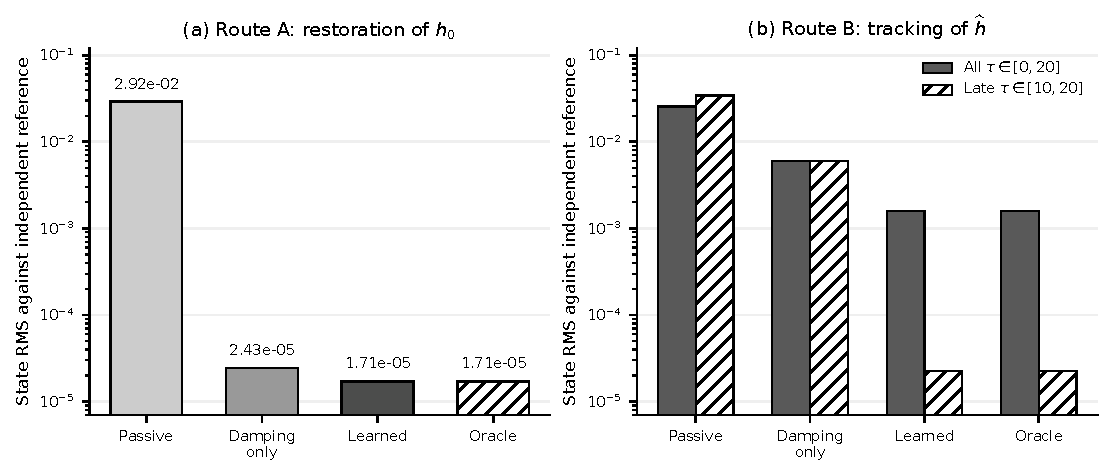
\includegraphics[width=\textwidth]{figures/new_baseline_results.pdf}
\caption{New-baseline comparisons using independent conservative
references. (a) Route A restores $h_0$ from the same initial state.
(b) Route B tracks a frozen $\widehat h$ trajectory from a nonzero
initial offset. Whole-window and late-window errors expose the tracking
transient. The panels compare different reference objects; their bars
are not a ranking of one route against the other.}
\label{num:results}
\end{figure*}

\subsection{Route-B prediction and tracking protocol}
\label{sx:route-b}
The route-B script regenerates the same training and validation data
and checks its newly fitted coefficient vector against the route-A
vector within $10^{-13}$. It then evaluates three conservative
trajectories, for $h_0$, $\widehat h$ and $h_*$, using RK4 step
$0.00025$ from the common initial state to $\tau=20$.
The prediction errors compare $h_0$ and $\widehat h$ with $h_*$;
the latter is synthetic ground truth, not independent physical data.
The $\widehat h$ and $h_*$ references are each checked against an
RK4 calculation at step $0.0005$.

For feedback, the reference is the frozen conservative $\widehat h$
flow, initialized at $(0.09,0.08,0.015,-0.01)$.
The actual initial state is $(0.0945,0.084,0.015,-0.01)$.
The position offset is $5\%$ of each reference position coordinate,
with zero momentum offset. The gains are $\kappa_p=1$, $\kappa_d=2$ in
dimensionless time. Passive, fitted damping-only, fitted tracking
and oracle tracking groups use this same reference. The learned
and oracle commands are the distinct laws in
\eqref{struct:route-b-control} and \eqref{struct:route-b-oracle}; the oracle uses true plant coefficients
for cancellation but retains the fitted reference trajectory.

The four actual-state variables and four reference variables form an
eight-dimensional midpoint solve with the same Newton settings as
\eqref{sx:newton-stop}. The independent RK4 trajectory is not fed into
that controller. It is used afterward to report the integration
component in \eqref{num:reference-split}.
A separate run halves the midpoint step to $0.0005$; the actual-state
maximum common-time difference is $2.22701\times10^{-5}$ and the
reference error falls by the factor $3.999984$.
A finite-difference check of the analytic augmented Jacobian has
maximum discrepancy $3.6902\times10^{-11}$ in the recorded check.
These finite differences are an implementation diagnostic, not a
replacement for the derived Jacobian.

For the oracle, the initial momentum-error vector is zero and the
continuous error satisfies
$e_X(\tau)=(1+\tau)e^{-\tau}e_X(0)$ and
$e_Y(\tau)=-\tau e^{-\tau}\mathsf N^{-1}e_X(0)$.
The discrete error is also compared with the independently formed
Cayley update of that linear system. The comparison tests the
feedback and reference coupling with a known error equation.


\subsection{Tracking sensitivity and combined archived displays}
\label{xtr:shared-results}
The five damping settings use the same fresh observations and fits as the
restoration tests in Supplementary Section~\ref{sx:damping}. Their tracking
runs last $\tau=10$, with midpoint step $0.002$ and independent RK4 step
$0.00025$; the late tracking window is $[5,10]$. These are independent fits
at each declared damping value, not one frozen controller exposed to
unknown changing damping. The following table retains both targets to
make their distinct time windows explicit.

\begin{table*}[t]
\centering
\caption{Independent-reference state RMS in the damping scan.
The two routes use distinct target Hamiltonians and time windows.}
\label{sx:damping-errors}
\begin{tabular}{rcccc}
\toprule
$\zeta_1^{\mathrm{d}}$ & A passive, $[0,10]$ & A learned, $[0,10]$ & B passive, $[5,10]$ & B learned, $[5,10]$\\
\midrule
$0$ & $3.77362\times10^{-5}$ & $3.42885\times10^{-5}$ & $6.02444\times10^{-3}$ & $1.09567\times10^{-4}$ \\
$0.01$ & $6.73657\times10^{-3}$ & $3.42885\times10^{-5}$ & $3.71321\times10^{-3}$ & $1.09567\times10^{-4}$ \\
$0.025$ & $1.59501\times10^{-2}$ & $3.42885\times10^{-5}$ & $1.62063\times10^{-2}$ & $1.09567\times10^{-4}$ \\
$0.05$ & $2.92396\times10^{-2}$ & $3.42885\times10^{-5}$ & $3.42497\times10^{-2}$ & $1.09567\times10^{-4}$ \\
$0.1$ & $4.97374\times10^{-2}$ & $3.42885\times10^{-5}$ & $6.13727\times10^{-2}$ & $1.09567\times10^{-4}$ \\
\bottomrule
\end{tabular}
\end{table*}

\begin{figure*}[t]
\centering
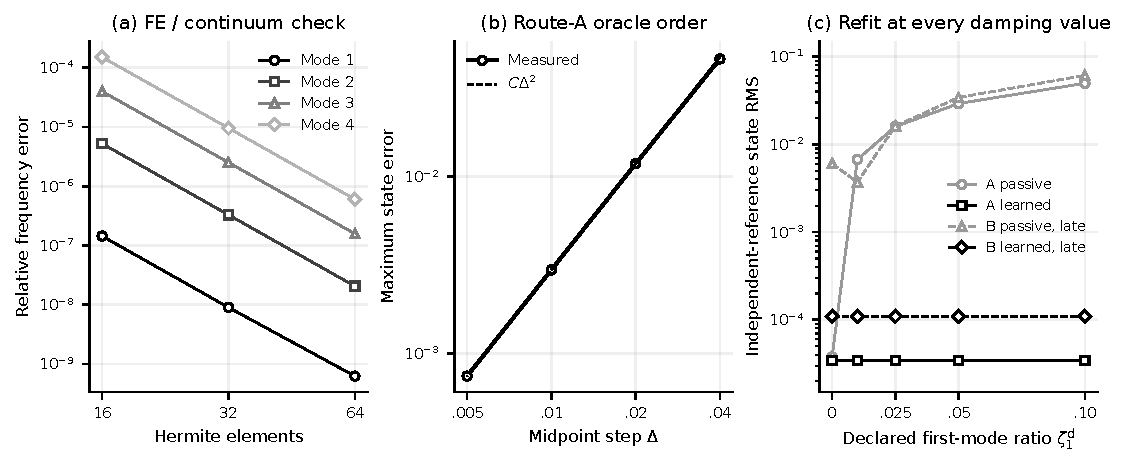
\includegraphics[width=\textwidth]{figures/new_baseline_verification.pdf}
\caption{Independent numerical checks from the supplied JSON records.
(a) The first four FE frequencies converge to roots of the continuum
endpoint determinant. (b) Route-A oracle errors converge at second
order against an independent RK4 reference. (c) Each damping setting
is refitted before either route is evaluated; A uses the full $[0,10]$
window and B the late $[5,10]$ window. Lines connect tested settings
and do not represent additional simulations or statistical intervals.}
\label{num:verification}
\end{figure*}
\begin{table*}[t]
\centering
\caption{Sampled local magnetic demand for the supplementary learned tracking test. This is an ideal command requirement, not a hardware capability measurement.}
\label{xtr:port-table}
\begin{tabular}{lcccc}
\toprule
Test & $\max|B_y|$ (mT) & $\max|B|$ (mT) & $\max\|\nabla B\|_2$ (T/m) & $\max|F_y|$ ($\mu$N)\\
\midrule
B: learned & $2.197941$ & $30.080408$ & $0.03453753$ & $0.611950$ \\
\bottomrule
\end{tabular}
\end{table*}

\clearpage
\begin{thebibliography}{99}

\bibitem[Abbott et~al.(2020)]{abbott}
Abbott JJ, Diller E and Petruska AJ (2020) Magnetic methods in robotics.
\textit{Annual Review of Control, Robotics, and Autonomous Systems} 3: 57--90.
\doi{10.1146/annurev-control-081219-082713}

\bibitem[Antman(2005)]{antman}
Antman SS (2005) \textit{Nonlinear Problems of Elasticity}. 2nd ed. Springer.
\doi{10.1007/0-387-27649-1}

\bibitem[Chen et~al.(2022)]{chen2022}
Chen Y, Matsubara T and Yaguchi T (2022) KAM theory meets statistical learning theory:
Hamiltonian neural networks with non-zero training loss.
\textit{Proceedings of the AAAI Conference on Artificial Intelligence} 36(6): 6322--6332.
\doi{10.1609/aaai.v36i6.20582}

\bibitem[Cho et~al.(2021)]{cho2021pdms}
Cho HS, Moon HY, Lee HS, Kim YT and Jeoung SC (2021) Formulation prediction for Young's modulus of poly(dimethylsiloxane) by spectroscopic methods.
\textit{Bulletin of the Korean Chemical Society} 42(9): 1225--1231. \doi{10.1002/bkcs.12352}

\bibitem[Desai et~al.(2021)]{desai}
Desai SA, Mattheakis M, Sondak D, Protopapas P and Roberts SJ (2021)
Port-Hamiltonian neural networks for learning explicit time-dependent dynamical systems.
\textit{Physical Review E} 104: 034312. \doi{10.1103/PhysRevE.104.034312}

\bibitem[Feng and Qin(2010)]{fengqin}
Feng K and Qin M (2010) \textit{Symplectic Geometric Algorithms for Hamiltonian Systems}. Springer.
\doi{10.1007/978-3-642-01777-3}

\bibitem[Feng et~al.(1989)]{feng}
Feng K, Wu HM, Qin MZ and Wang DL (1989) Construction of canonical difference
schemes for Hamiltonian formalism via generating functions.
\textit{Journal of Computational Mathematics} 7(1): 71--96.
\url{https://computmath.cjoe.ac.cn/jcm/EN/Y1989/V7/I1/71}.

\bibitem[Fischer et~al.(2017)]{fischer2017adhesion}
Fischer SCL, Kruttwig K, Bandmann V, Hensel R and Arzt E (2017) Adhesion and cellular compatibility of silicone-based skin adhesives.
\textit{Macromolecular Materials and Engineering} 302(5): 1600526. \doi{10.1002/mame.201600526}

\bibitem[Francescon et~al.(2025)]{francescon2025shape}
Francescon V, Murasovs N, Lloyd P, Onaizah O, Chathuranga DS and Valdastri P (2025)
Closed-loop shape-forming control of a magnetic soft continuum robot.
\textit{IEEE Robotics and Automation Letters} 10(6): 6071--6078.
\doi{10.1109/LRA.2025.3565124}

\bibitem[Greydanus et~al.(2019)]{greydanus}
Greydanus S, Dzamba M and Yosinski J (2019) Hamiltonian neural networks.
In: \textit{Advances in Neural Information Processing Systems}, vol. 32.
\url{https://arxiv.org/abs/1906.01563}.

\bibitem[Hairer et~al.(2006)]{hairer}
Hairer E, Lubich C and Wanner G (2006) \textit{Geometric Numerical Integration:
Structure-Preserving Algorithms for Ordinary Differential Equations}. 2nd ed. Springer.
\doi{10.1007/3-540-30666-8}

\bibitem[Haro and Luque(2019)]{haro2019aposteriori}
Haro \`A and Luque A (2019) A-posteriori KAM theory with optimal estimates for
partially integrable systems. \textit{Journal of Differential Equations}
266(2--3): 1605--1674. \doi{10.1016/j.jde.2018.08.003}
Preprint version used: \url{https://arxiv.org/abs/1711.05515v1}.

\bibitem[Hornik(1991)]{hornik}
Hornik K (1991) Approximation capabilities of multilayer feedforward networks.
\textit{Neural Networks} 4(2): 251--257. \doi{10.1016/0893-6080(91)90009-T}

\bibitem[Kim et~al.(2019)]{kim}
Kim Y, Parada GA, Liu S and Zhao X (2019) Ferromagnetic soft continuum robots.
\textit{Science Robotics} 4(33): eaax7329. \doi{10.1126/scirobotics.aax7329}

\bibitem[K\&J Magnetics(2026)]{kjMoment}
K\&J Magnetics (accessed 28 October 2026) Magnetic dipole moment.
\url{https://www.kjmagnetics.com/blog/magnetic-dipole-moment}.
Engineering dipole-moment approximation.

\bibitem[Lussi et~al.(2021)]{lussi2021cvs}
Lussi J et~al. (2021) A submillimeter continuous variable stiffness catheter for compliance control.
\textit{Advanced Science} 8(18): 2101290. \doi{10.1002/advs.202101290}

\bibitem[P\"oschel(2001)]{poschel}
P\"oschel J (2001) A lecture on the classical KAM theorem.
In: \textit{Proceedings of Symposia in Pure Mathematics}, vol. 69, pp. 707--732.
\doi{10.1090/pspum/069/1858551}
Preprint version used: \url{https://arxiv.org/abs/0908.2234v1} (Version 1.3, 2009).

\bibitem[Shang(1999)]{shang}
Shang ZJ (1999) KAM theorem of symplectic algorithms for Hamiltonian systems.
\textit{Numerische Mathematik} 83: 477--496. \doi{10.1007/s002110050460}

\bibitem[Simo(1985)]{simo}
Simo JC (1985) A finite strain beam formulation. The three-dimensional dynamic problem.
Part I. \textit{Computer Methods in Applied Mechanics and Engineering} 49(1): 55--70.
\doi{10.1016/0045-7825(85)90050-7}

\bibitem[SM Magnetics(2026)]{smN50}
SM Magnetics / SuperMagnetMan (accessed 28 October 2026) Magnet material grades: NdFeB stock grades, N50.
\url{https://supermagnetman.com/pages/magnet-material-grades}.
Manufacturer grade range, not an individual magnet calibration.

\bibitem[Su et~al.(2007)]{su2007}
Su HL, Sun YJ, Qin MZ and Scherer R (2007) Structure preserving schemes for Birkhoffian systems.
\textit{International Journal of Pure and Applied Mathematics} 40(3): 341--366.
\url{https://www.ijpam.eu/contents/2007-40-3/4/4.pdf}.

\bibitem[Tong et~al.(2025)]{tong2025navigation}
Tong D, Hao Z, Li J, Sun B, Liu M, Wang L and Huang W (2025)
Real-time simulation enabled navigation control of magnetic soft continuum robots in confined lumens.
\textit{Journal of the Mechanics and Physics of Solids} 203: 106198.
\doi{10.1016/j.jmps.2025.106198}

\bibitem[Trabelsi et~al.(2018)]{trabelsi}
Trabelsi C, Bilaniuk O, Zhang Y et~al. (2018) Deep complex networks.
In: \textit{International Conference on Learning Representations}.
\url{https://arxiv.org/abs/1705.09792}.

\bibitem[Zhang et~al.(2022)]{zhang}
Zhang SQ, Gao W and Zhou ZH (2022) Towards understanding theoretical advantages of
complex-reaction networks. \textit{Neural Networks} 151: 80--93.
\doi{10.1016/j.neunet.2022.03.024}
\href{https://www.lamda.nju.edu.cn/zhangsq/papers/2022-CRNet-NN.pdf}{Published version used for theorem numbering}.

\bibitem[Zhong et~al.(2020)]{zhong}
Zhong YD, Dey B and Chakraborty A (2020) Dissipative SymODEN: Encoding Hamiltonian
dynamics with dissipation and control into deep learning.
In: \textit{ICLR Workshop on Integration of Deep Neural Models and Differential Equations}.
\url{https://arxiv.org/abs/2002.08860}.
\end{thebibliography}

\end{document}
